
\section{  EXAMPLES OF LSST SCIENCE PROJECTS                    }
\label{Sec:science}

The design and optimization of the LSST system leverages its unique capability
to scan a large sky area to a faint flux limit in a short amount of time.
The main product of the LSST system will be a multi-color $ugrizy$ image of about
half the sky to unprecedented depth ($r\sim27.5$). For a comparison, the best
analogous contemporary dataset is that of SDSS, which provides $ugriz$ images
of about a quarter of the sky to $r\sim22.5$, with twice as large seeing
(see Figs.~\ref{Fig:panels1} and \ref{Fig:panels2}). A major advantage of LSST
is the fact that this deep sky map will be produced by taking hundreds of
shorter exposures (see Table~\ref{tab:baseline}). Each sky position within the main survey area
will be observed about 1000 times, with time scales spanning seven orders of
magnitude (from 30 sec to 10 years), and produce over \textit{a trillion
photometric measures} of celestial sources.

It is not possible to predict all the science that LSST data will enable.
We now briefly discuss a few projects to give a flavor of anticipated studies,
organized by the four science themes that drive the LSST design
(although some projects span more than one theme).
\B{For an in-depth discussion of LSST science cases, we refer the reader to the
LSST Science Book.}


\vskip 0.3in
\subsection{Probing Dark Energy and Dark Matter }

A unique aspect of LSST as a probe of dark energy and dark matter is
the use of multiple cross-checking probes that reach unprecedented
precision (see Fig.~\ref{Fig:DEellipses}). Any given probe constrains
degenerate combinations of cosmological parameters, and each probe is
affected by different systematics, thus the combination of probes
allows systematics to be calibrated and for degeneracies to be
broken.  Dark energy manifests itself in two ways.  The first is the
relationship between redshift and distance (the Hubble diagram), or
equivalently the expansion rate of the Universe as a function of
cosmic time.  The second is the rate at which matter clusters with
time.
Structure formation involves a balance between
gravitational attraction of matter over-densities and the rapid
expansion of the background.  Thus, quantifying the rate of growth of
structures from early times until the present provides additional
tests of the energy contents of the Universe and their interactions.

The joint analysis of LSST weak lensing and galaxy clustering is
particularly powerful in constraining the dynamical behavior of dark
energy, i.e., how it evolves with cosmic time or redshift \citep{2004PhRvD..70D3009H,2006JCAP...08..008Z}.  By
simultaneously measuring the growth of large-scale structure, and
luminosity and angular distances as functions of redshift (via weak
lensing, LSS, SN, and cluster counting), LSST data can reveal whether
the recent cosmic acceleration is due to dark energy or modified
gravity \citep{2004PhRvD..69D4005L,2006PhRvD..74B3512K,2006PhRvD..74d3513I,2008PhRvD..78f3503J,2011PhRvD..83b3008O,2013ApJ...779...39J,Weinberg2013}.
The Dark Energy Survey \citep[see e.g.,][and references therein]{2017arXiv170801530D} provides a compelling proof of concept for this program.

Over a broad range of accessible redshifts, the simple linear model
for the dark energy equation of state ($w = w_0 + w_a(1-a)$) is a poor representation of more
general dark energy theories. \citet{2008PhRvD..78d3528B} showed that in a high-dimensional dark energy model space,
LSST data could lead to a hundred- to thousand-fold increase in precision over its
precursor experiments, thereby confirming its status as
a premier Stage IV experiment in the sense of \citet{2006astro.ph..9591A}.
%Fits of multi-parameter dark energy models to the complementary LSST
%probes of dark energy will constrain alternative models of gravity.

The power and accuracy of LSST dark energy and dark matter probes are
a result of the enormous samples that LSST will have, including
several billion galaxies and millions of Type Ia
supernovae. At $i < 25.3$ (SNR${}>20$ for point sources), the
photometry of galaxies will be of high enough quality to provide
photometric redshifts with an RMS accuracy ($\sigma/(1+z)$) of 1-2\%
over the range $0.3 < z < 3.0$ (only
10\% of the sample will have redshift errors larger than 4\%).
This number represents a requirement on the accuracy of the photometry at delivering photometric
redshifts given known templates for the SEDs.  The degradation in photometric redshift quality associated without having more
training data than currently exists to define the template set increases the
expected $\sigma/(1+z)$ to $\sim$0.05 \cite[e.g.][]{2015APh....63...81N,2017arXiv170609507G}, which is still well within the
expected range for a Stage IV dark energy experiment.  The
sample to this depth will include several billion galaxies.  At a
slightly brighter cut, there will be around 30 galaxies arcmin$^{-2}$
with shapes measured well enough for weak lensing measurements \citep{2013MNRAS.434.2121C,2015MNRAS.447.1746C},
with the number realized in practice being dependent on
the performance of the deblending and shape measurement algorithms.
The median redshift for
this sample will be $z\sim$1.2, with the third quartile at $z\sim2$.
It will be possible to further improve photometric redshift calibration
by cross-correlating the photometric sample with redshift surveys of
galaxies and quasars in the same fields
\citep{2008ApJ...684...88N,2010ApJ...721..456M,2013arXiv1303.4722M,2017arXiv171002517D}.


\begin{figure}
%\includegraphics[width=1.0\hsize,clip]{DEellipses1.pdf}
%\includegraphics[width=0.95\hsize,clip]{DEellipses2.pdf}
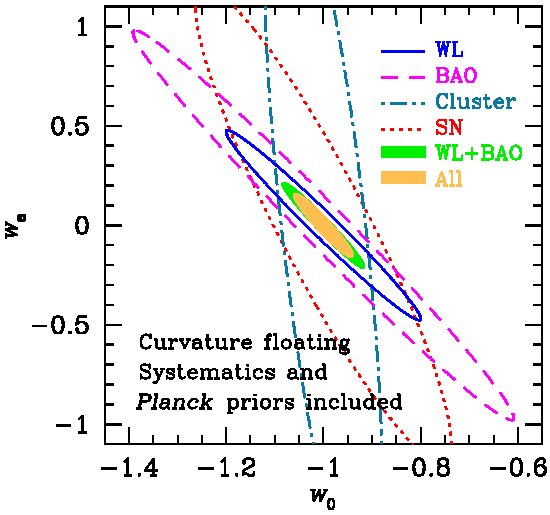
\includegraphics[width=1.0\hsize,clip]{cswb.pdf}
\caption{
Constraints on the dark energy equation of state ($w = w_0 +
w_a(1-a)$) from LSST cosmological probes.  The various ellipses assume
constraints from BAO (dashed line), cluster counting (dash-dotted line),
supernovae (dotted line), WL (solid line), joint BAO and WL
(green shaded area), and all probes combined (yellow shaded area).
The BAO and WL results are based on galaxy--galaxy, galaxy--shear,
and shear--shear power spectra only.
Adding other probes such as strong lensing time delay
and higher-order galaxy and shear statistics will further improve
the constraints.  While some survey parameters mentioned in the text differ slightly from
those in the LSST Science Book (which were used to make this figure), changing the size of the
contours for individual probes, the key point remains that
this combination of dark energy probes results in contours with different degeneracy directions, and
hence their combination results in tight constraints on the dark energy equation of state. }
\label{Fig:DEellipses}
\end{figure}



% \begin{figure}
% 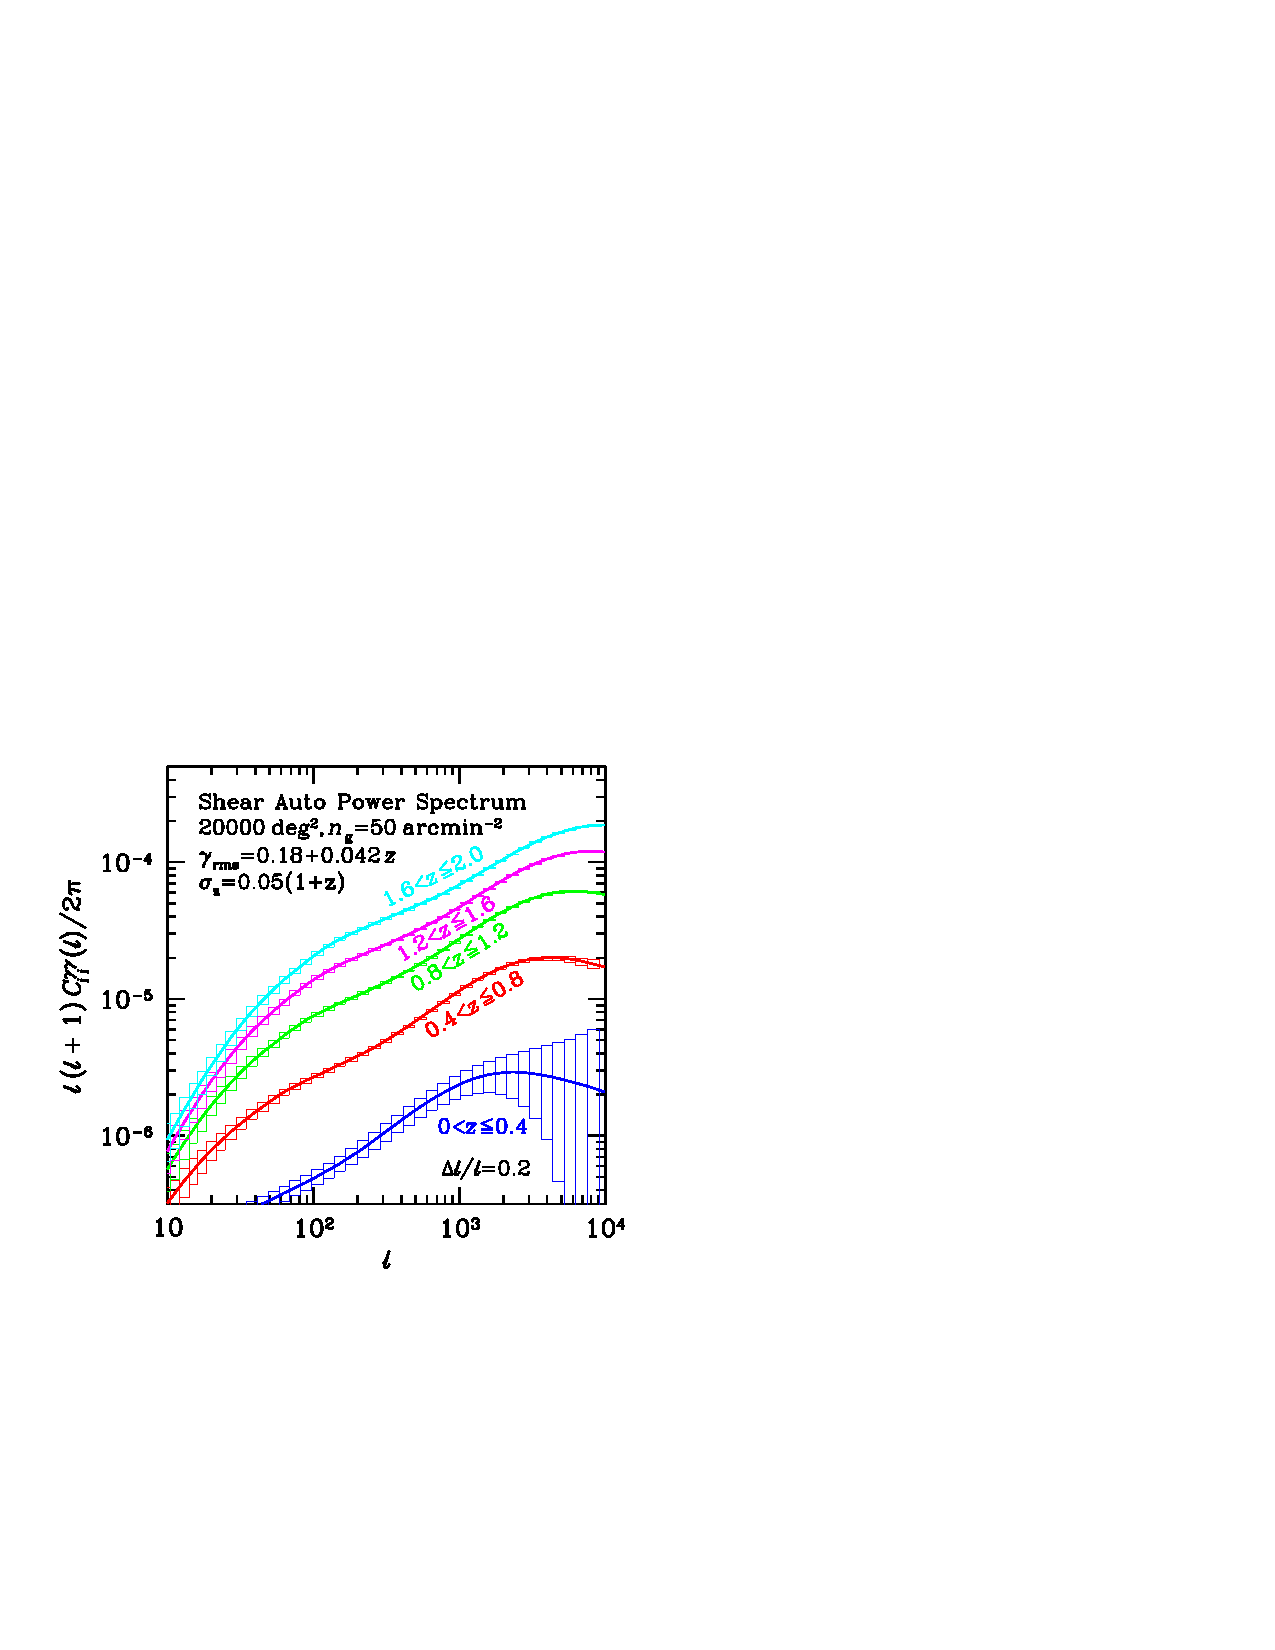
\includegraphics[width=1.0\hsize,clip]{cls.pdf}
% \caption{The lensing shear auto power spectra constructed from 5 redshift bins
% ($l$ is the multipole moment of the distribution on the sky). Only the 5 auto-power
% spectra of each redshift bin among the available 15 cospectra are displayed, and the
% solid curves show the predictions for the concordance $\Lambda$CDM model. The boxes
% show the expected 1-$\sigma$ measurement error (in bins of $\Delta l/l=0.2$) from the full LSST
% 10-year survey due to the sample (i.e., cosmic) variance which dominates at about
% $l< 100$, and intrinsic ellipticities which dominate at $l> 1000$ \citep{2006JCAP...08..008Z}.}
% \label{Fig:wlPk}
% \end{figure}


%\begin{figure}
%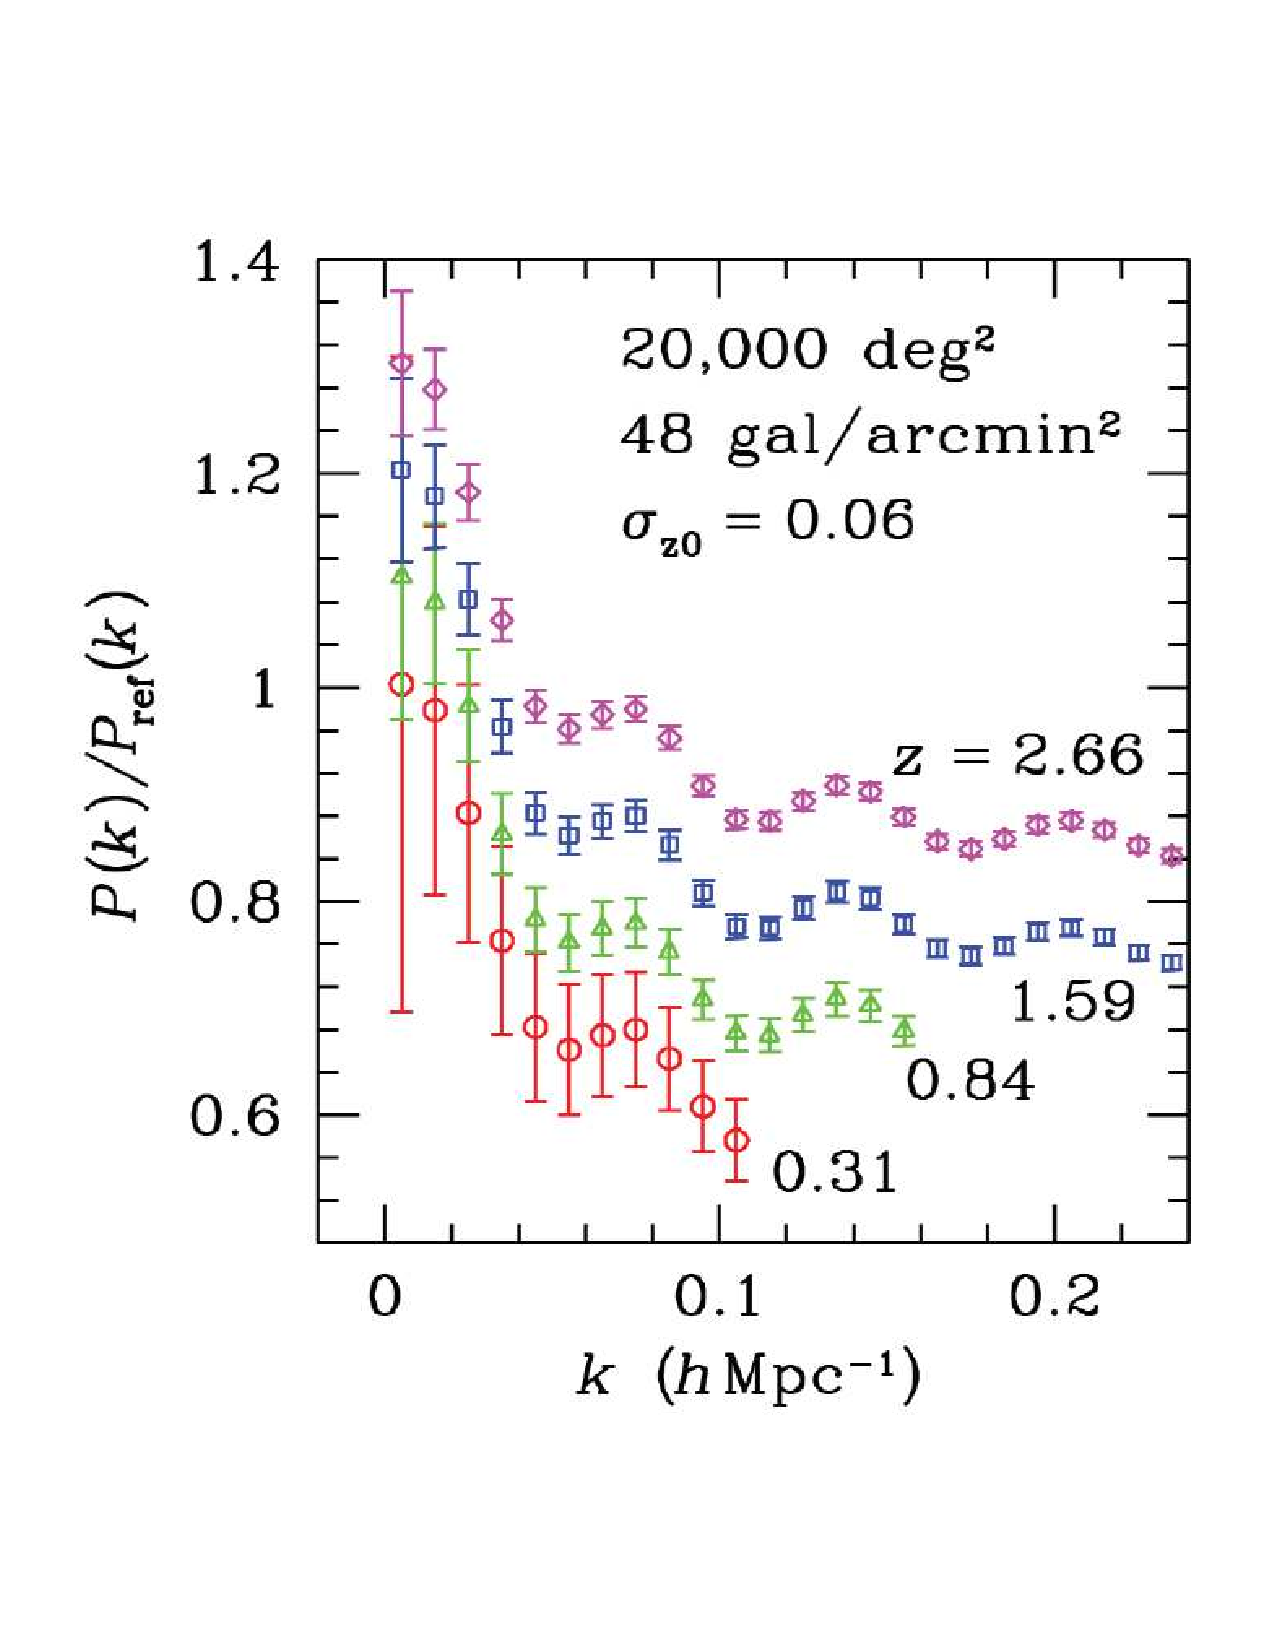
\includegraphics[width=1.0\hsize,clip]{bao.pdf}
%\caption{Simulations of the ratio of the measured galaxy power spectrum to
%a featureless reference power spectrum in various redshift bins (shifted vertically
%for clarity), for the full LSST survey using conservative photometric redshift
%errors. The several peaks visible in each curve are the signature of baryon acoustic
%oscillations \citep{2005ApJ...633..560E,2005MNRAS.362..505C,2014MNRAS.441...24A}. LSST will measure the
%angular diameter distance over this redshift range with an accuracy of $\sim1$\%
%\citep{2006ApJ...644..663Z}.}
%\label{Fig:bao}
%\end{figure}



\begin{figure}
%\includegraphics[width=1.0\hsize,clip]{dgcon.pdf}
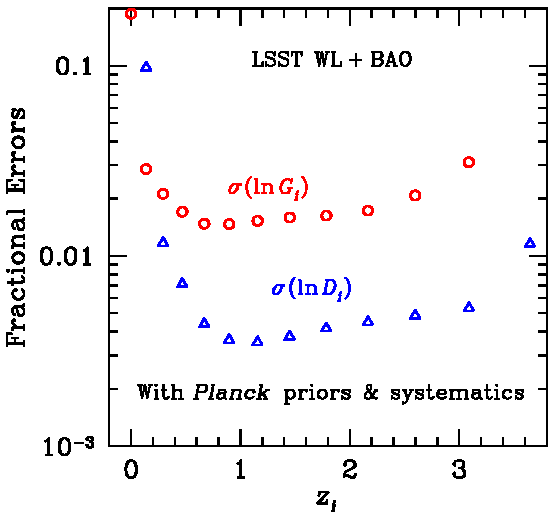
\includegraphics[width=1.0\hsize,clip]{dges.pdf}
\caption{Marginalized $1\sigma$ errors on the comoving distance
(open triangles) and growth factor (open circles) parameters from
the joint analysis of LSST LSS and WL (galaxy--galaxy, galaxy--shear,
and shear--shear power spectra) with a
conservative level of systematic uncertainties in the photometric redshift error
distribution and additive and multiplicative errors in the shear and
galaxy power spectra. The maximum multipole used for WL is
2000, and that for LSS is 3000 [with the additional requirement that
$\Delta_\delta^2(\ell/D_{A};z) < 0.4$].
The growth parameters
%, $G_0 \ldots G_{14}$,
are evenly spaced in
$\log(1+z)$ between $z = 0$ and 5, and the distance parameters
%$D_1 \ldots D_{14}$,
start at $z_1 = 0.14$.
% (see text for details).
The error of each distance (growth) parameter is marginalized
over all the other parameters including growth (distance) parameters. The joint constraints on
distance are relatively insensitive to the assumed systematics
\citep{2009ApJ...690..923Z}.}
\label{Fig:bao2}
\end{figure}


The main LSST observables in the context of dark energy and matter are described below.

\begin{itemize}
\item The \textsl{3x2-point} joint analysis of shear--shear, galaxy--shear, and galaxy--galaxy
correlation functions has become standard in analyses of precursor datasets
\cite[e.g.][]{2017arXiv170801530D,2017arXiv170706627J}. WL and LSS are highly complementary probes, and the combination
of their auto- and cross-correlations will constrain the properties of the late-time accelerated expansion while providing
internal cross-checks for marginalizing over systematic uncertainties \cite[e.g.,][]{2017arXiv171003235M}.
These measurements consist of the two-point auto- and cross-correlations of shear and positions for billions of galaxies across $\sim 10$ redshift bins.
As described in the following two items, the galaxy-galaxy and galaxy-shear correlation functions provide additional probes of dark energy and dark matter.
%\item Measurements of the two-point auto- and cross-correlation of shear across multiple redshift bins.
%(Fig.~\ref{Fig:wlPk}).
% There will be over 50 of these auto and cross power spectra constructed from the shape catalog with excellent photometric redshifts
% \citep{2003PhRvL..91n1302J}.
%
%\item The shear--shear correlation function, often referred to as ``cosmic shear,'' provides a direct probe of the
%underlying matter distribution ([best citation?]) and is independent of the galaxy bias. The growth of structure can be
%measured with photometric redshift tomography. These correlations can also be used to construct mass maps which
%enable numerous cross-correlation studies.
%
\item The galaxy--shear correlation function probes the growth of dark matter large-scale structure and is a
diagnostic of the underlying cosmology. The combination with the
galaxy--velocity correlation function estimated from spectroscopic observations of millions of galaxies
could probe General Relativity at high redshift \citep{Reyes2007}.
%
\item The galaxy--galaxy correlation function is vital to constrain the galaxy bias impacting the galaxy-shear correlation and is therefore
an essential component in the joint analysis of LSS and WL. In addition, the presence of
Baryon Acoustic Oscillations in the galaxy angular correlation functions is a strong cosmological
probe on its own. The sound horizon at decoupling, which is imprinted on the
mass distribution at all redshifts and calibrated with the CMB, provides a standard ruler to measure the angular diameter
distance as a function of redshift
\citep[Fig.~\ref{Fig:bao};][]{1998ApJ...504L..57E,2001ApJ...557L...7C,2003ApJ...594..665B,2003PhRvD..68f3004H,2003PhRvD..68h3504L,2003ApJ...598..720S}.
LSST photo-$z$ BAO will achieve percent-level precision on the angular
diameter distance at $\sim$10 redshifts logarithmically spaced between $z = 0.4$ to 3.6. The combination with CMB
and weak lensing (WL) shear yields tight constraints on the
dynamical behavior of dark energy (Fig.~\ref{Fig:bao2}). In particular, high-redshift BAO data can break
the degeneracy between curvature and dark energy, constraining $\Omega_k$ to within
0.001.
%, which is about ten times better than the most accurate current
%result based on WMAP and SDSS data \citep{2009ApJS..180..330K,2010MNRAS.401.2148P}.
%I TOOK THIS OUT; THIS CONSTRAINT IS COMPARABLE TO THAT OF PLANCK.
\item Higher-order shear and galaxy statistics and shear peak counts can improve dark energy
constraints and provide self-calibration of various systematics
\citep{2004MNRAS.348..897T,2006MNRAS.366..884D,2006MNRAS.366..101H,2016PhRvD..94f3534P}. They are also probes of both
primordial non-Gaussianities and those caused by non-linear structure.
\item Primordial non-Gaussianity is also probed by the large-scale power of any biased tracer of the matter
overdensities \citep{2008PhRvD..77l3514D}. Although measurements of the galaxy power spectrum on very large scales
are challenging due to sky systematics \citep{2014PhRvL.113v1301L} and cosmic variance, the prospect of using
multiple tracers of the same field could significantly improve the constraining power for this observable
\citep{2009PhRvL.102b1302S}. Similar measurements of the large-scale power will also be used to test for phenomenological
models of clustering dark energy \citep{2006PhRvD..74d3505T}.
\item Similarly, weak lensing magnification tomography \citep{2012MNRAS.426.2489M} offers a
complementary probe of a mix of cosmic geometry and growth of dark matter structure.
\item The two LSST observing programs are complementary in the supernova samples they will provide. 1) The main survey will
obtain light curves in six bands and photometric redshifts of about 400,000 photometrically-classified Type
Ia supernovae that can be used for cosmological distance measurements, with further spectroscopic
follow-up of a sub-sample of their host galaxies.
Such a sample will not only provide larger statistics
for the study of the Type Ia population in the universe, but will also be spread across a large sky
area of about 18,000 sq degrees allowing different probes of the large scale structure of the low redshift
universe. This sample of supernovae can be used as a tracer of large scale structure by directly probing the
gravitational potential of structure through inferences of their peculiar velocities
\citep{Gordon2007,2011PhRvD..83d3004B,2017ApJ...847..128H}, weak lensing of supernova brightnesses
\citep{2006PhRvD..74f3515D,2014PhRvD..89b3009Q,Macaulay2016,Scovacricchi2017}, and the local bulk flow
\citep{Reiss1999,2011JCAP...04..015D,2012MNRAS.420..447T,2013A&A...560A..90F,2015JCAP...12..033H} as well as
low redshift constraints on the isotropy of the universe \citep{Javanmardi2015,2010JCAP...12..012A,Campanelli2011,Cai2013,Colin2011}.
2) The rapidly sampled ``mini-survey''
(deep drilling field) of selected areas, possibly coadded over short time scales,  will yield well-sampled
light curves of tens of thousands of supernovae to redshifts peaking around $z\sim 0.7$ and reaching beyond a
redshift of 1.0, limited by the systematics related to the limits of our astrophysical understanding of supernovae
populations and relative photometric calibration. Such a deep drilling sample will constrain cosmological parameters
through the standardizable candle property of supernova Type Ia, as well as through correlations in measured
luminosities probing large scale structures, as the deep drilling fields are also of larger spatial area compared
to earlier supernova surveys. The ultimate promise of such supernova surveys will be linked to the observing strategy employed by the LSST.
\item Unique constraints on anisotropy of cosmological parameters over the sky using, which will test fundamental cosmological
assumptions of homogeneity and isotropy.
For example, WL$+$LSS and SN can separately probe anisotropy of dark energy \citep[e.g.,][]{2009ApJ...690..923Z}.
\item The shape of the power spectrum of dark matter fluctuations measured by LSST weak lensing
will constrain the sum of neutrino masses with an accuracy
of 0.04 eV or better \citep{1999A&A...348...31C,2004PhRvD..70f3510S,2006JCAP...06..025H}.
%The current best limit, as derived from a combination of WMAP, the SDSS power spectrum,
%SN, and the Ly$\alpha$ forest, is 0.17 eV \citep{Seljak2006}.
\item Tens of thousands of galaxy-galaxy lenses will provide the needed statistics to probe dark matter
halo profiles and substructure \cite[e.g.,][]{2006MNRAS.368..715M,2012Natur.481..341V}. The image fluxes in several thousand well-measured
strongly lensed quasars will enable constraints of the dark matter mass function on small scales \citep{2002ApJ...572...25D}.
\item The abundance of galaxy clusters as a function of mass and redshift is sensitive to cosmological parameters
\citep[SciBook, Ch.~13;][]{2014MNRAS.443.1973V}. LSST will produce a large catalog of clusters detected through their member galaxy population
to redshift $z\sim 1.2$.  In addition, LSST will identify optical counterparts and provide deep optical
imaging for clusters detected in other wavebands \citep[e.g.,][]{2009ApJ...701...32S}.
\item The clustering properties of those same galaxy clusters will also be used to constrain
  cosmological parameters \citep{1996MNRAS.282.1096M,2013MNRAS.434..684M}, to marginalize over uncertainties in
  the mass-observable relation and photometric redshift uncertainties \citep{2011PhRvD..83b3008O}, and to constrain the effects of super-sample covariance in the two-point functions of WL and LSS \citep{2003ApJ...584..702H,2014MNRAS.441.2456T}.
%\item The distribution of strongest WL shear peaks with redshift is
%  closely related to the galaxy cluster abundance, but has the
%  potential to be a more robust and more directly calibratable statistic. This is a simultaneous
%probe of the universal mass function and the growth of structure, and provides a useful
%constraint on dark energy \citep{2005astro.ph.12513W}. LSST will find over 200,000 such
%shear peaks on galaxy cluster scales.
%% Note from RM: removed that point.  We now know that we need alternate ways to calibrate a variety
%% of effects (projection, etc.) and in practice we will have those alternate measurements for
%% optical clusters, but not for shear peaks.  The distribution of peaks down to lower S/N is likely
%% still a useful probe, but peak-counting for clusters is not competitive.
\item LSST will discover several hundred galaxy clusters that produce multiple-image lenses of background objects.
Cluster mass reconstruction based on the multiple image positions
 can probe the cluster inner mass profile, and can provide a separate test of cosmology, especially
in cases with strongly lensed background objects at different redshift \citep{2000ApJ...532..679P,2003MNRAS.338L..25O}.
\item Time delays of galaxy-scale lensed quasars will allow one to measure Hubble's constant
\citep[e.g.,][]{2010ApJ...711..201S,2017MNRAS.465.4914B} in hundreds of systems; sub-percent level precision in
$H(z)$ should be achievable \citep{2009ApJ...706...45C,2016A&ARv..24...11T}, providing a further independent dark energy probe.
LSST will also discover between 500 and 1000 strongly lensed Type Ia supernovae \citep{2017ApJ...834L...5G,2017arXiv170800003G}, which will provide hundreds of additional high-quality time delays.
Time delays for quasars multiply lensed by clusters as a function of redshift are an independent test
of dark energy \citep{1997ApJ...482...75K}. The natural timescale (many months to years) is well matched
to the LSST survey \citep{2010MNRAS.405.2579O}.
\item Standard sirens are a new cosmological probe, demonstrated by the recent discovery of a binary
  neutron star merger by LIGO with an electromagnetic counterpart \citep{2017ApJ...848L..12A}, which was
  used to constrain the Hubble parameter to roughly 15\% precision \citep{2017arXiv171005835A}.
  Constraints from standard sirens are independent of the local distance ladder, with the primary
  uncertainties being the local velocity field and the inclination angle of the system.  \citet{2017arXiv171005845S}
  estimate of order 70 such systems could be found with LSST.
\end{itemize}


\subsection{Taking an Inventory of the Solar System}



The small bodies of the Solar System, such as main-belt asteroids,
the Trojan populations of the giant planets and the Kuiper Belt objects,
offer a unique insight into its early stages because they provide
samples of the original solid materials of the solar nebula.
Understanding these populations, both physically and in their number
and size distribution, is a key element in testing various theories of
Solar System formation and evolution.

The baseline LSST cadence will result in orbital parameters for several
million objects; these will be dominated by main-belt asteroids, with
light curves and multi-color photometry for a substantial fraction of detected objects.
This dataset will yield 10 to 100 times more objects than are currently
available with orbits, colors, and variability information. LSST will make a significant contribution the Congressional target
completeness of 90\% for PHAs larger than 140 m (\S~\ref{Sec:NEOc}), and will detect over 30,000 TNOs brighter than $r\sim24.5$ using its baseline cadence. LSST will be capable
of detecting objects like Sedna to beyond 100 AU, thus enabling \textit{in situ} exploration
far beyond the edge of the Kuiper belt at $\sim$50 AU. Because most of these
objects will be observed several hundred times, accurate orbital elements,
colors, and variability information will also be available.


\begin{figure}
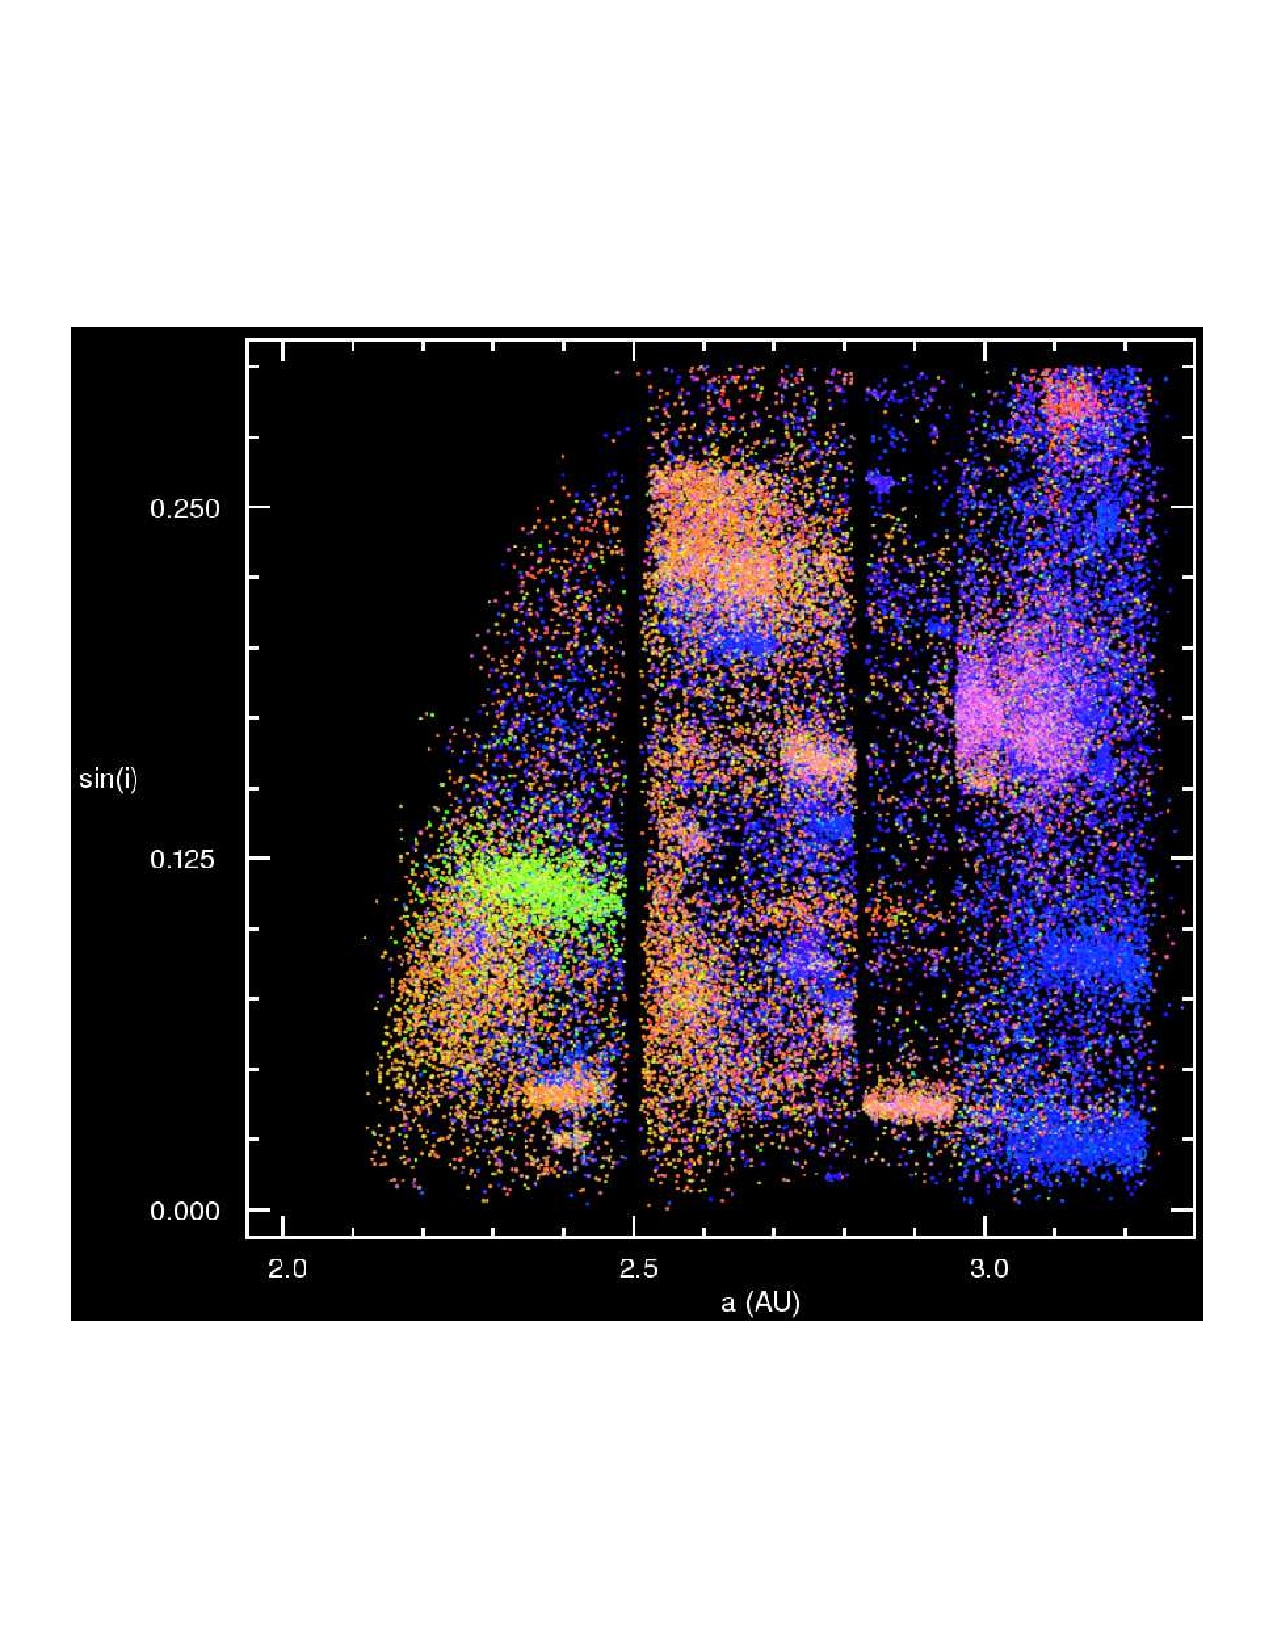
\includegraphics[width=1.0\hsize,clip]{asteroids.pdf}
\caption{An example of color-based asteroid taxonomy. The figure
shows the distribution of asteroids in the proper semi-major axis vs. $\sin(i)$
plane for 45,000 asteroids with colors measured by SDSS \citep{2008Icar..198..138P}.
The color of each dot is representative of the object's color.
Note the strong correlation between asteroid families (objects in distinct regions
of the plane) and colors. There are
at least five different taxonomic types distinguishable with SDSS measurements;
LSST color measurements of asteroids will be more than twice as accurate
and will increase the number of objects by roughly two orders of magnitude.}
\label{Fig:asteroids}
\end{figure}

\begin{figure}
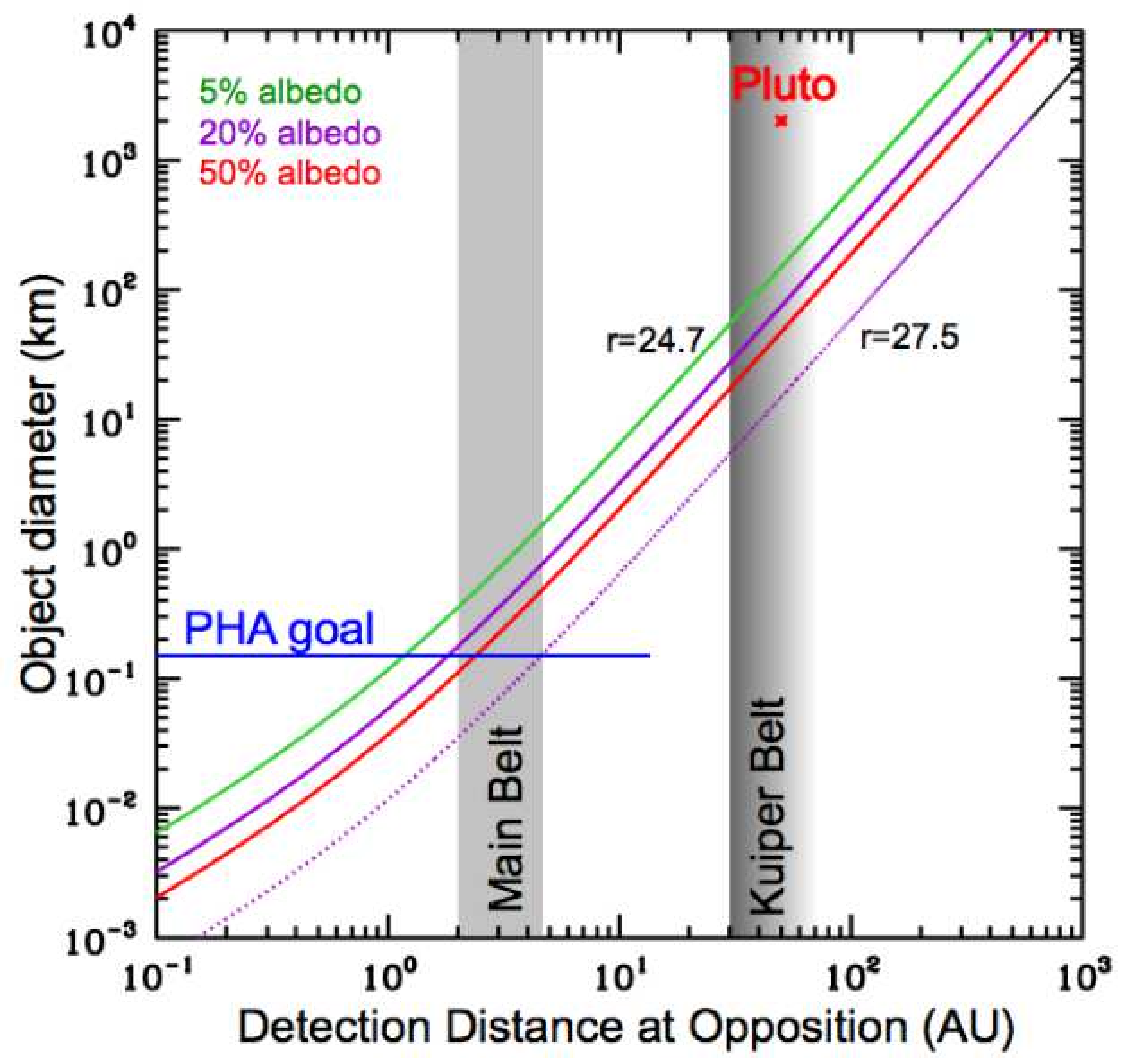
\includegraphics[width=1.0\hsize,clip]{Af9.pdf}
\caption{The LSST detection limits for distant Solar System objects as
  a function of distance.
Moving objects with diameters as small as 100m in the main asteroid belt and
100km in the Kuiper Belt (TNOs) will be detected in individual visits,
depending on the albedo. Specialized deeper observations
(see \S~\ref{Sec:minisurveys}) will detect TNOs as small as 10 km. Adapted from
\citet{2007AAS...21113714J}.}
\label{Fig:Af9}
\end{figure}



The following are some examples of the LSST science opportunities in
Solar System science:
\begin{itemize}
\item Studies of the distribution of orbital elements for over 5 million main-belt
asteroids as a function of color-based taxonomy (see Fig.~\ref{Fig:asteroids})
and size; size distributions of asteroid families \citep{2008Icar..198..138P} and their
correlations with age \citep{2004Natur.429..275J,2005Icar..173..132N}; dynamical
effects \citep{2001Sci...294.1693B}; and studies of object shapes and spin states using
light curve inversion techniques \citep{2000Icar..148...12P,2009A&A...493..291D}.
\item Studies of transient activity in asteroids (active asteroids or main belt comets,
\citet{2006Sci...312..561H}),  due to mass loss with associated extended
morphology.  Only a few such objects are currently known \citep{2011AJ....142...28J,2012AJ....143...66J};
LSST
will increase the sample of such objects to $\sim$100.
\item Studies of the distribution of orbital elements for about 100,000 NEOs as a
function of color and size \citep{1993ApJ...407..412R,2003Icar..163..363D};
correlations with the analogous distributions for
main-belt objects, and studies of object shapes and structure using light curves.
\item Studies of the distribution of orbital elements for close to 300,000 Jovian Trojan
asteroids as a function of color and size \citep{2000AJ....120.1140J,2005AJ....130.2900Y,2007MNRAS.377.1393S};
the search for dynamical families
\citep{2005HiA....13..758K}; studies of shapes and structure using light curves.
\item Studies of the distribution of orbital elements for about 30,000 TNOs (see
Fig.~\ref{Fig:Af9}) as a function of color and size; the search for dynamical families
\citep{2011ApJ...733...40M}; studies of shapes and structure using light curves
\citep{1995AJ....110.3073D,2001AJ....122..457T,2001AJ....122.1051G,2004AJ....128.1364B,2005AJ....129.1117E,2006Icar..185..508J,2007AJ....134.2186D}.
\item An unbiased and complete census of both Jupiter-family and Oort-cloud
comets; six-band sub-arcsecond spatial profiles to a faint surface brightness
limit; temporally resolved activity \citep{1999A&A...349..649L,2004come.book...17A}.
\item Searching for objects with perihelia out to several hundred AU. For example, an object
like Sedna \citep{2004ApJ...617..645B} would be detectable at 130 AU. This will result
in a much larger, well-understood sample of inner Oort Cloud objects like Sedna and 2012 VP113
 \citep{2014Natur.507..471T}.  Studying the distribution of their orbits (in particular including any
clustering in the argument of perihelion) will test models predicting the existence of a planetary-mass object beyond Neptune, a proposed Planet 9 \citep{2014Natur.507..471T,2016AJ....151...22B,2016ApJ...824L..23B,2016AJ....152..221S,2017AJ....154...65B}. Depending on the proposed Planet 9's on-sky location and brightness, it may be possible for LSST to directly detect it in the wide survey images \citep{2016AJ....151...22B,2016ApJ...824L..23B,2016AJ....152..221S,2017AJ....154...65B}.

\item Mapping the propagation of interplanetary coronal mass ejections using induced
 activity in a large sample of comets at different heliocentric distances
(SciBook Ch.~5).
\item Probing the inventory and frequency of  interstellar asteroids/comets. The recent discovery of interstellar object
1I/2017 U1 (`Oumuamua), discovered by the Panoramic Survey Telescope and Rapid Response System (Pan-STARRS1) \citep{2017MPEC....U..181B}, has shown the power  of large, complete all-sky surveys to unearth
rare and exciting classes of objects. LSST will be some three magnitudes more sensitive
than  current NEO surveys (like Pan-STARRS1), and cover more sky more
often. Therefore, LSST is likely to find more interstellar objects, and more frequently.
Estimates from  \citet{2016ApJ...825...51C},  \citet{2017AJ....153..133E}, and \citet{2017ApJ...850L..38T} suggest that LSST will increase the number of  such rare objects by an order of magnitude which, among other outcomes, will help
constrain the frequency and properties of planetary system formation in the solar neighborhood.
\end{itemize}


\subsection{ Exploring the Transient Optical Sky }




\begin{figure}
\hskip -0.1in
\vskip -0.1in
%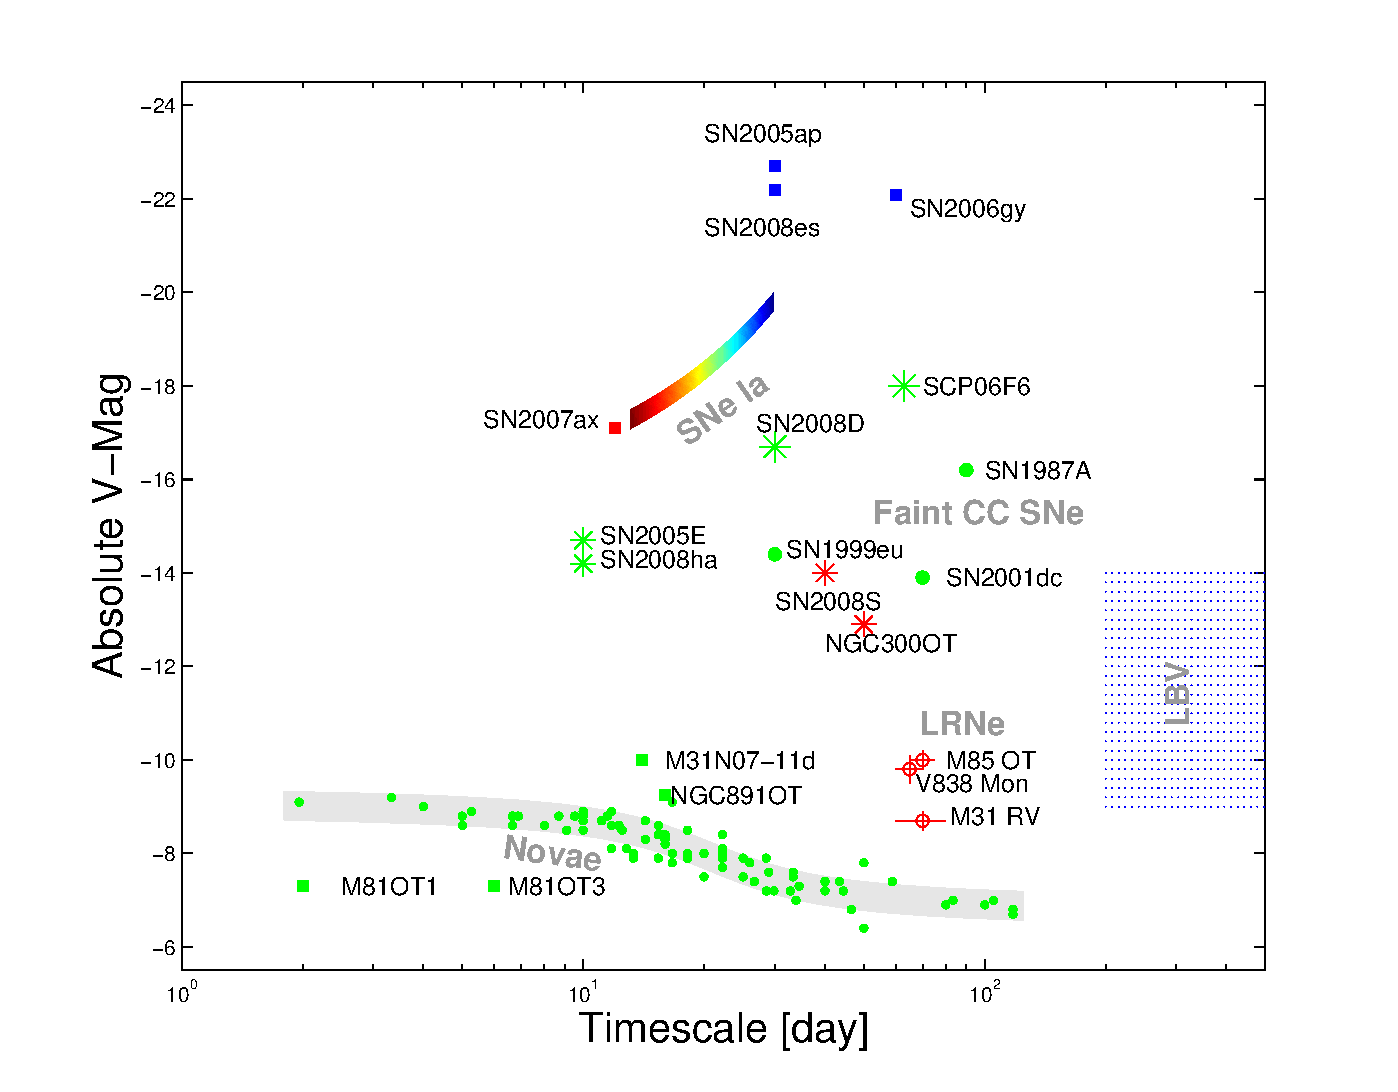
\includegraphics[width=1.1\hsize,clip]{shri2.pdf}
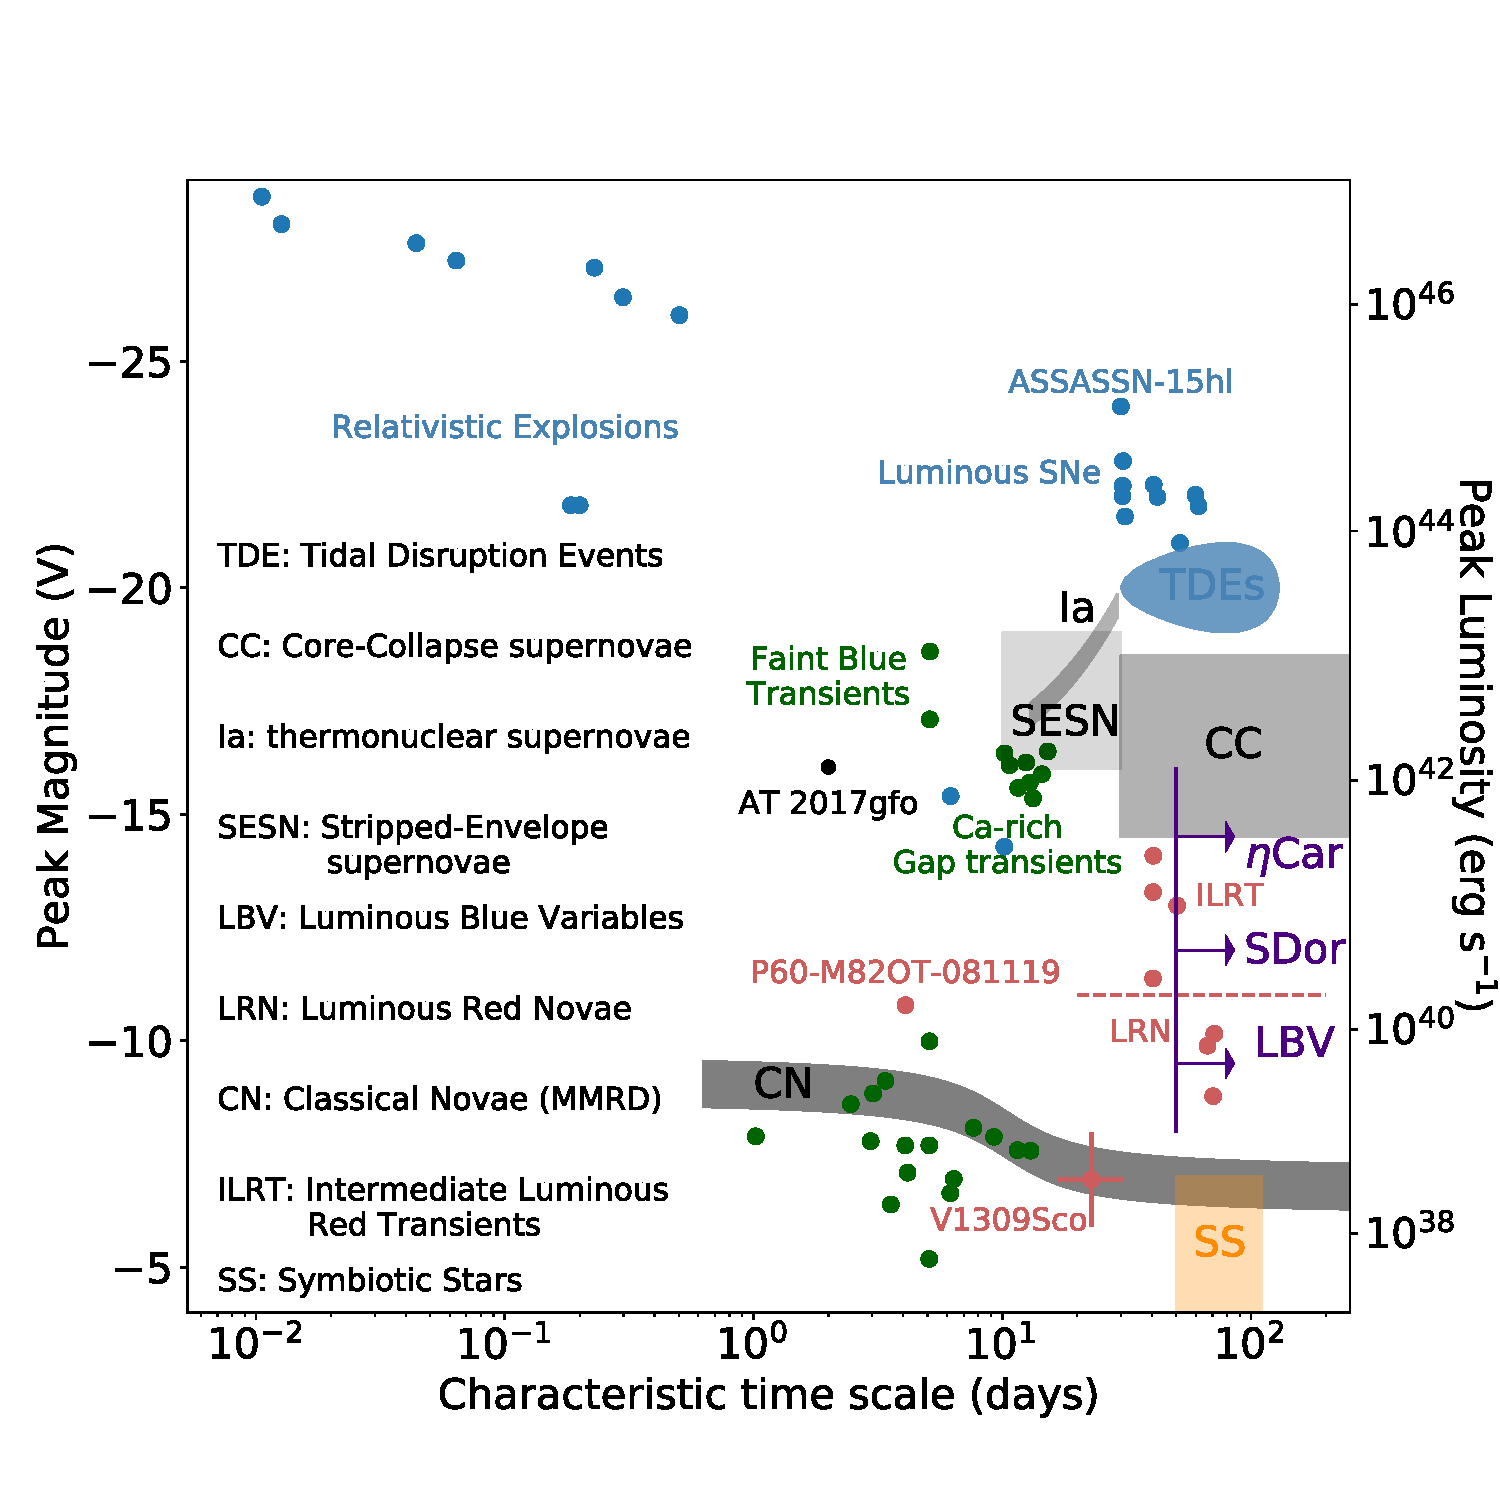
\includegraphics[width=1.0\hsize,clip]{taumv_updated.pdf}
%\vskip -0.1in
\caption{The phase space of cosmic explosive and eruptive transients
  as represented by their absolute $V$ band peak brightness and the
  event timescale, defined as the time taken to drop one magnitude in
  V band brightness from peak luminosity (adapted from \citet{2007Natur.447..458K}
  and \citet{2011PhDT........35K}).  The locus of the Classical
  Novae (MMRD) is as described in \citet{DellaValle1995}.  LSST
  will open up large regions of this phase space for systematic
  exploration by extending time-volume space over 100 times over
  existing surveys.}
\label{Fig:shri}
\end{figure}

Time domain science will greatly benefit from LSST's unique capability
to simultaneously provide large area coverage, dense temporal
coverage, accurate color information, good image quality, and rapid
data reduction and classification. Since LSST extends time-volume
space more than one hundred times over current surveys \citep[e.g.,][]{2008ApJ...676..163M}
it will facilitate new population and statistical studies and also the discovery of new classes of
objects.  LSST data products will enable many projects including:

\begin{itemize}


\item Discovery and characterization of thousands of hot Jupiters
  in exoplanetary systems via the transit method \citep{2012ApJ...753..160W}.
LSST will extend the extrasolar planet census to larger distances within the Galaxy, thus enabling detailed studies
of planet frequency as a function of stellar metallicity and parent population \cite[e.g.,][]{2009ApJ...695..336H,2011ApJ...743..103B}.
The out-of-transit variability of exoplanet host stars will also provide characterization of the system
via flaring behavior and stellar age via gyrochronology, the latter helping constrain theories of tidal evolution and
migration in giant planets.

\item Gravitational microlensing in the Milky Way \cite[see][]{2008ApJ...681..806H} as well as in the Local Group and beyond \citep{2008A&A...478..755D}.

\item Studies of dwarf novae, including their use as probes of stellar populations and
      structure in the Local Group \citep{2005AJ....129.1873N,2006AJ....131.2980S,2009ApJ...692..324S}. Population studies of the end points of binary evolution differentiating long orbital period vs short orbital period dwarf novae at different places in the galaxy, as well as the numbers of recurrent vs normal novae. Regular cadence, long term color observation on a large sample of galactic sources will enable the identification of CVs containing highly magnetic white dwarfs, that are red due to cyclotron emission from the magnetic accretion column and in low state for the majority of the 10-year survey.

\item Studies of  transients from poorly-constrained stages of stellar evolution including
stellar eruptions,  luminous blue variable (LBV), stellar mergers, and helium core flashes leading to white dwarf formation,  both through pre-eruption characterization of sources at the positions of eruptive transients in the deep LSST stacks and detection of faint precursor eruptions, and by constraining rates of individual eruption subclasses \citep{2014ARA&A..52..487S} and detecting them in galaxies out to tens of Mpc.

\item A census of light echoes of historical explosive and eruptive
  transients in the Milky Way and Local Group through high resolution
  time series.

\item Studies of known and unusual SN populations and parameterization of their light curves \citep[e.g.,][]{1998ApJ...495..617H,2003ApJ...590..944W,2007ApJ...667L..37H,2008ApJ...686..749K,2009ApJ...700.1097H,2012ApJ...748..127F,2014ApJS..213...19B,2017Natur.551..210A}, including late-time observations of rapidly-evolving transients to deep limits, critical for ascertaining their nature. Measurements of intrinsic rates for both peculiar transients \cite[e.g.,][]{2014ApJ...794...23D} and for SN as a function of sub-type and host environment properties \citep[e.g., metallicity;][]{2017ApJ...837..120G}.

\item A deep search for new populations of novae and supernova progenitors
      \citep[][see Fig.\ref{Fig:shri}]{2009ARA&A..47...63S,2009ApJ...705.1364T,2011MNRAS.415..773S} both through direct imaging and through the detection of SN precursor events \citep{2013Natur.494...65O}, characterization of pre-SN variability of SN progenitors and the frequency of pre-SN outbursts.

\item The discovery of strongly lensed SNe; $500-1000$ multiply imaged SN~Ia \citep{2017ApJ...834L...5G,2017arXiv170800003G}
and at least several hundred strongly lensed core-collapse SNe \citep{2010MNRAS.405.2579O}
are expected to be discovered by LSST. Time delays between the multiple images of strongly lensed core-collapse
SNe can be used to observe the elusive shock breakout phase of the light curve, providing an unprecedented look
at the earliest emission from these transients \citep{2017arXiv171100183S}.

\item A large, well characterized sample of super luminous supernovae
including object at redshift as high as $z=2.5$, a sample large enough to be leveraged for cosmology  improving constraints on $w$ and $\Omega_m$ \citep{Scovacricchi2015}.

\item Studies of optical bursters (those varying faster than 1 mag hr$^{-1}$) to $r\sim25$ mag.

\item Detection and measurement of gamma-ray burst afterglows and transients
      \cite[e.g.,][]{2004IJMPA..19.2385Z,2006ApJ...642..354Z,2010ApJ...720.1513K} to high redshift ($\sim$7.5).

\item Large scale studies of stellar tidal disruptions by nuclear supermassive
  black holes \cite[e.g.,][]{1989ApJ...346L..13E,2008ApJ...676..944G,2009MNRAS.400.2070S,2011Sci...333..203B,2012EPJWC..3903001G,2015JHEAp...7..148K}, as well as binary
  supermassive black holes in the in-spiral phase \cite[e.g.,][]{2009MNRAS.393.1423C,2017MNRAS.465.3840C}.
  Persistent observations leading to complete (except for
  seasonal gaps) lightcurve of long duration events like
  TDEs. Measurements of rates as function of galaxy type, redshift,
  and level of nuclear activity. An assessment of the diversity
  of these events in terms of total power, effective temperature, and
  jet launching efficiency.


\item A study of quasar variability using accurate, multicolor light
  curves for a few million
quasars, leading to constraints on the accretion physics and nuclear environments \citep{2003AJ....126.1217D,2004ApJ...601..692V,2010ApJ...721.1014M,2017ApJ...836..186J}.
      Relations between quasar variability
      properties and luminosity, redshift,
      rest-frame wavelength, time scale, color, radio-jet emission, black-hole
      mass, and Eddington-normalized luminosity will be defined with massive
      statistics, including the potential to detect rare but important events such as
      jet flares and obscuration events. Microlensing events will also be monitored in the $\sim$4000 gravitationally-lensed
      quasars discovered by LSST and used to measure the spatial structure of quasar accretion disks.

\item The superb continuum light curves of AGN will enable economical ``piggyback"
      reverberation-mapping efforts using spectroscopy of emission lines
      \cite[e.g.,][]{2012ApJ...747...62C,2015ApJS..216....4S,2017arXiv171103114G}. These results
      will greatly broaden the luminosity-redshift plane of reverberation-mapped AGNs
      with black-hole mass estimates. For LSST data alone, the inter-band continuum lags
      will provide useful structural information.

\item Optical identification of transients and variables detected in
  other electromagnetic wavebands, from gamma rays to radio. Examples
  include optical and gamma ray variability in blazars \citep{2014MNRAS.439..690H},
  radio transients associated with tidal disruption flares
  \citep{2011MNRAS.416.2102G}, and radio counterparts to supernovae and
  GRBs \citep{2006ApJ...639..331G}. Deep optical observations with LSST may
  also help illuminate the nature of fast radio bursts \cite[FRBs,][]{2007Sci...318..777L,2013Sci...341...53T}.

\item Optical identification of counterparts to non-electromagnetic
  sources, such as gravitational waves (GW) and neutrino events
  (LIGO\footnote{http://www.ligo.caltech.edu},
  ICECUBE\footnote{http://icecube.wisc.edu}).  LSST's unique ability
  to characterize the faint variable sky over large areas will be
  important for the detection of GW associated sources, with an estimate
  of $\sim 7$ discoveries per year \citep{2017arXiv171005845S}.  The power
  of the Advanced LIGO (aLIGO)/Virgo\footnote{http://public.virgo-gw.eu/language/en/} experiment led to the discovery
  of four GW events in less than a year. The binary
  neutron star merger event GW170817 was accompanied by emission
  detected across the entire electromagnetic spectrum \citep{Abbott2017}.
  Multiple teams discovered bright UV/optical/NIR emission
  arising from the radioactive decay of heavy elements synthesized
  during the NS merger, a ``kilonova'' emission (SSS17a).  The
  evolution of the kilonova was somewhat unexpected \citep{Abbott2017}.
  The ${\sim100}$ kilonovae sample that LSST is expected to
  generate will enable comparative studies of these transients. LSST
  will also be important for eliminating potential false positives
  \citep{2013ApJ...767..124N,2012ApJ...746...48M}.

\end{itemize}


\subsection{Mapping the Milky Way }

The LSST will map the Galaxy in unprecedented detail, and by doing so revolutionize the fields of Galactic
Astronomy and Near-field Cosmology. The great detail with which the Milky Way can be studied complements
the statistical power of extra-galactic observations.  The overarching goal of near-field cosmology is to use
spatial, kinematic, and chemical data sets of stars to reveal the structure and evolution history of the Milky Way
and its environment. LSST will reveal this fossil record in great detail and provide a Rosetta Stone for extragalactic
astronomy by setting the context within which we interpret these
broader data sets. Moreover, different candidate supersymmetric
particle dark matter models predict different mass clustering on small
scales, and thus different mass functions for subhalos of the Milky
Way.  Thus the LSST census of faint satellites and stellar streams in
the halo will offer a unique means to constrain the
particle nature of dark matter.


\begin{figure}
%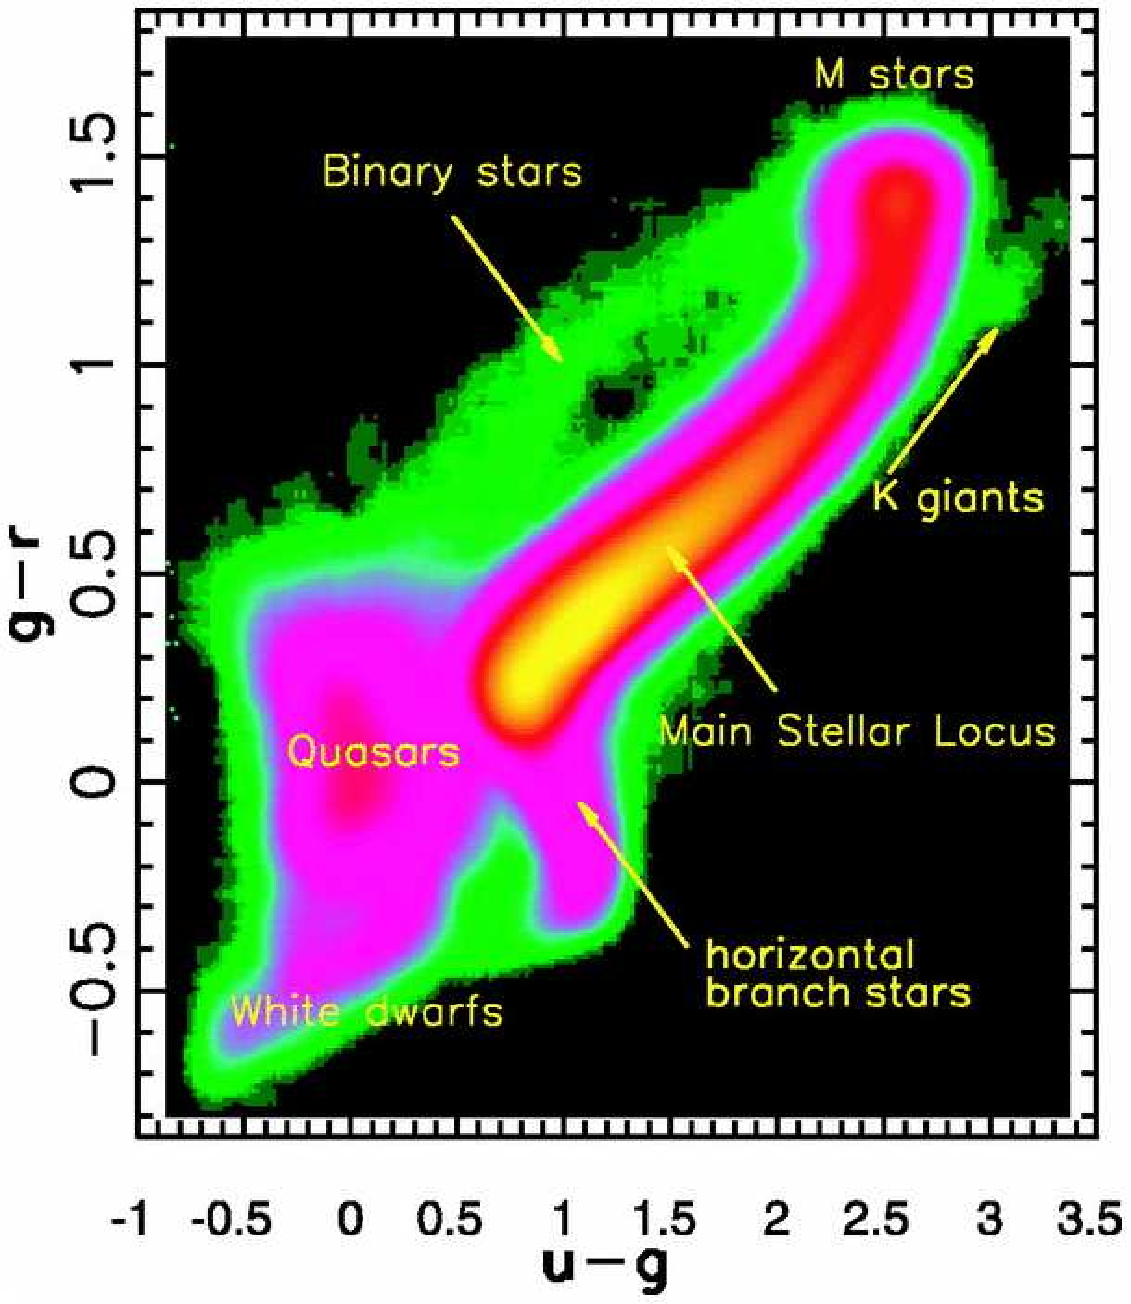
\includegraphics[width=1.0\hsize,clip]{smolcic.pdf}
%\hskip -1.0in
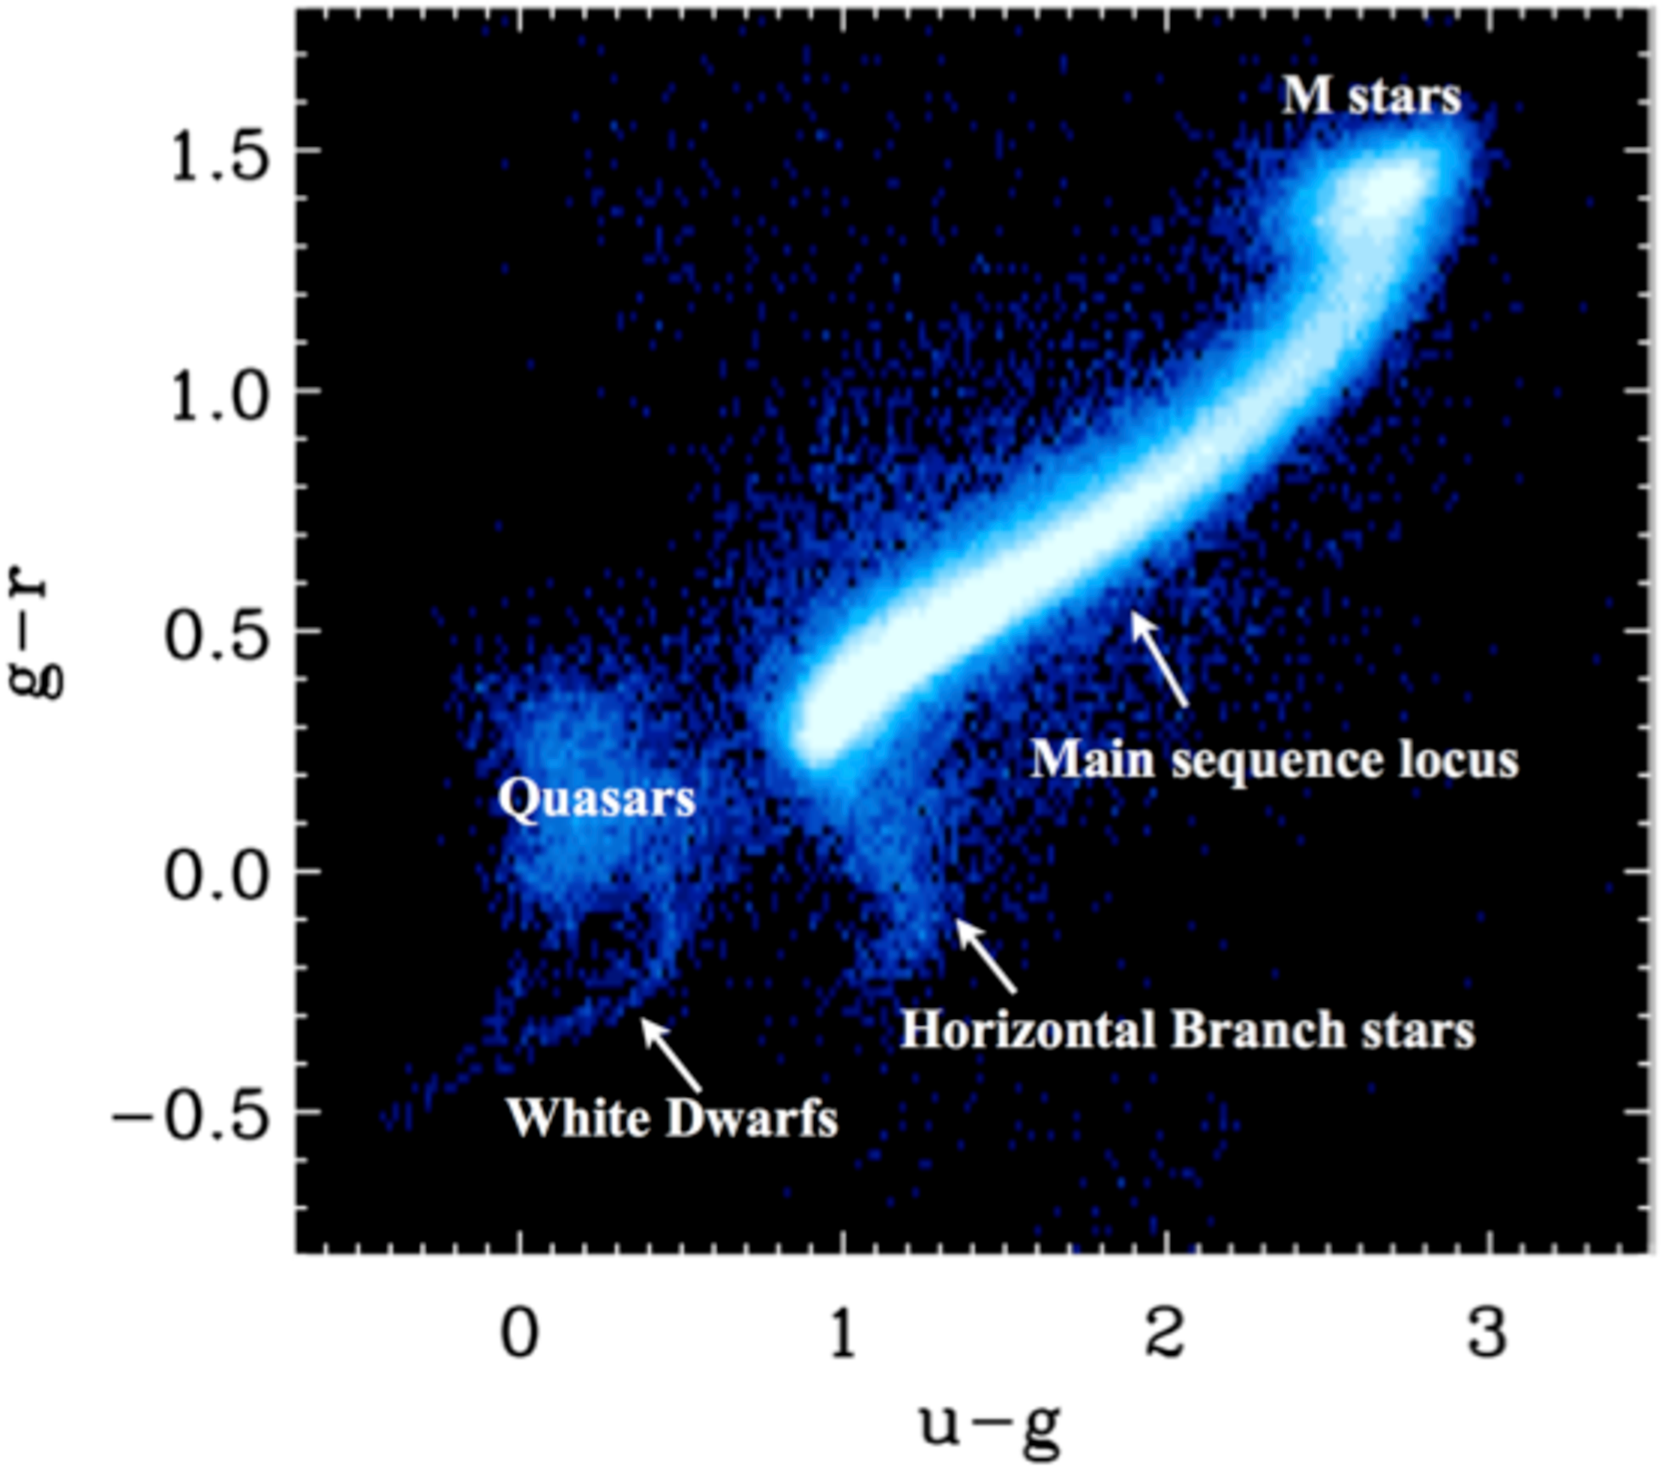
\includegraphics[width=1.0\hsize,clip]{MarlaUGR.pdf}
%\vskip -0.3in
\caption{The $g-r$ vs. $u-g$ color-color diagram for about a million points sources
from SDSS Stripe 82 area. Accurate multi-color photometry
contains information that can be used for source classification and determination of
detailed stellar properties such as effective temperature and metallicity. LSST will
enable such measurements for billions of stars.}
\label{Fig:FeH}
\end{figure}


The LSST will produce a massive and exquisitely accurate photometric and astrometric data set for about 20 billion
Milky Way stars. The coverage of the Galactic plane will yield data for numerous star-forming
regions, and the $y$ band data will penetrate through the interstellar dust layer. Photometric metallicity
measurements (see Figs.~\ref{Fig:FeH} and \ref{Fig:FeH3}) will be available for about 200 million main-sequence
F/G stars which will sample the halo to distances of 100 kpc \citep{2008ApJ...684..287I,2013ApJ...763...65A}. No other
existing or planned survey will provide such a powerful dataset to
study the outer halo: Gaia
is flux limited at $r=20$, and the Dark Energy Survey \citep{2011AJ....141..185R} and Pan-STARRS both
lack observations in the $u$ band, necessary for estimating metallicity. The LSST in its standard surveying mode will
be able to detect RR Lyrae variables (pulsating stars and standard candles) and classical novae (exploding stars
and standard candles) at a distance of 400 kpc and hence explore the extent and structure of our  halo out to
half the distance to the Andromeda galaxy. Thus, the LSST will enable studies of the distribution of main-sequence
stars beyond the presumed edge of the Galaxy's halo (see Fig.~\ref{Fig:halo}), of their metallicity distribution
throughout most of the halo, and of their kinematics beyond the thick disk/halo boundary. LSST will also obtain
direct distance measurements via trigonometric parallax below the hydrogen-burning limit for a representative
thin-disk sample.

% the SkyMapper \citep{Keller2001} which is flux limited to $r=22.6$
% (but will nicely complement SDSS in the Southern hemisphere),

In addition to the study of hydrogen burning stars, LSST will uncover the largest sample of stellar remnants to date.
Over 97\% of all stars eventually exhaust their fuel and cool to become white dwarfs. Given the age of the Galactic
halo, a significant fraction of the mass in this component may reside in these remnant stars
\citep[e.g.,][]{2000ApJ...542..281A,2007A&A...469..387T}
and therefore their discovery directly constrains the Galactic mass budget.  These large
populations of disk and halo white dwarfs will provide unprecedented constraints on the luminosity function of
these stars, which will directly yield independent ages for the Galactic disk and halo (e.g., through the initial-final mass
relation, \citet{2008ApJ...676..594K}).

The sky coverage of LSST naturally targets both field stars and star clusters.  To date, no systematic survey of the stellar
populations of Southern hemisphere clusters has been performed (e.g., such as the CFHT Open Star Cluster Survey, or
the WIYN Open Star Cluster Survey in the North; \citet{2001AJ....122..257K,2000ASPC..198..517M}).  Multiband imaging of these co-eval,
co-spatial, and iso-metallic systems will provide vital insights into fundamental stellar evolution.  For example, the depth
of LSST will enable construction of  luminosity and mass functions for nearby open clusters down to the hydrogen burning
limit and beyond.  Variations in the initial mass function will be studied as a function of environment (e.g., age and metallicity).
The wide-field coverage will also allow us to track how the stellar populations in each cluster vary as a function of radius,
from the core to beyond the tidal radius. Fainter remnant white dwarfs will be uncovered in both open and globular clusters
(the nearest of which are all in the South), thereby providing a crucial link to the properties of the now evolved stars in each
system.



\begin{figure}
%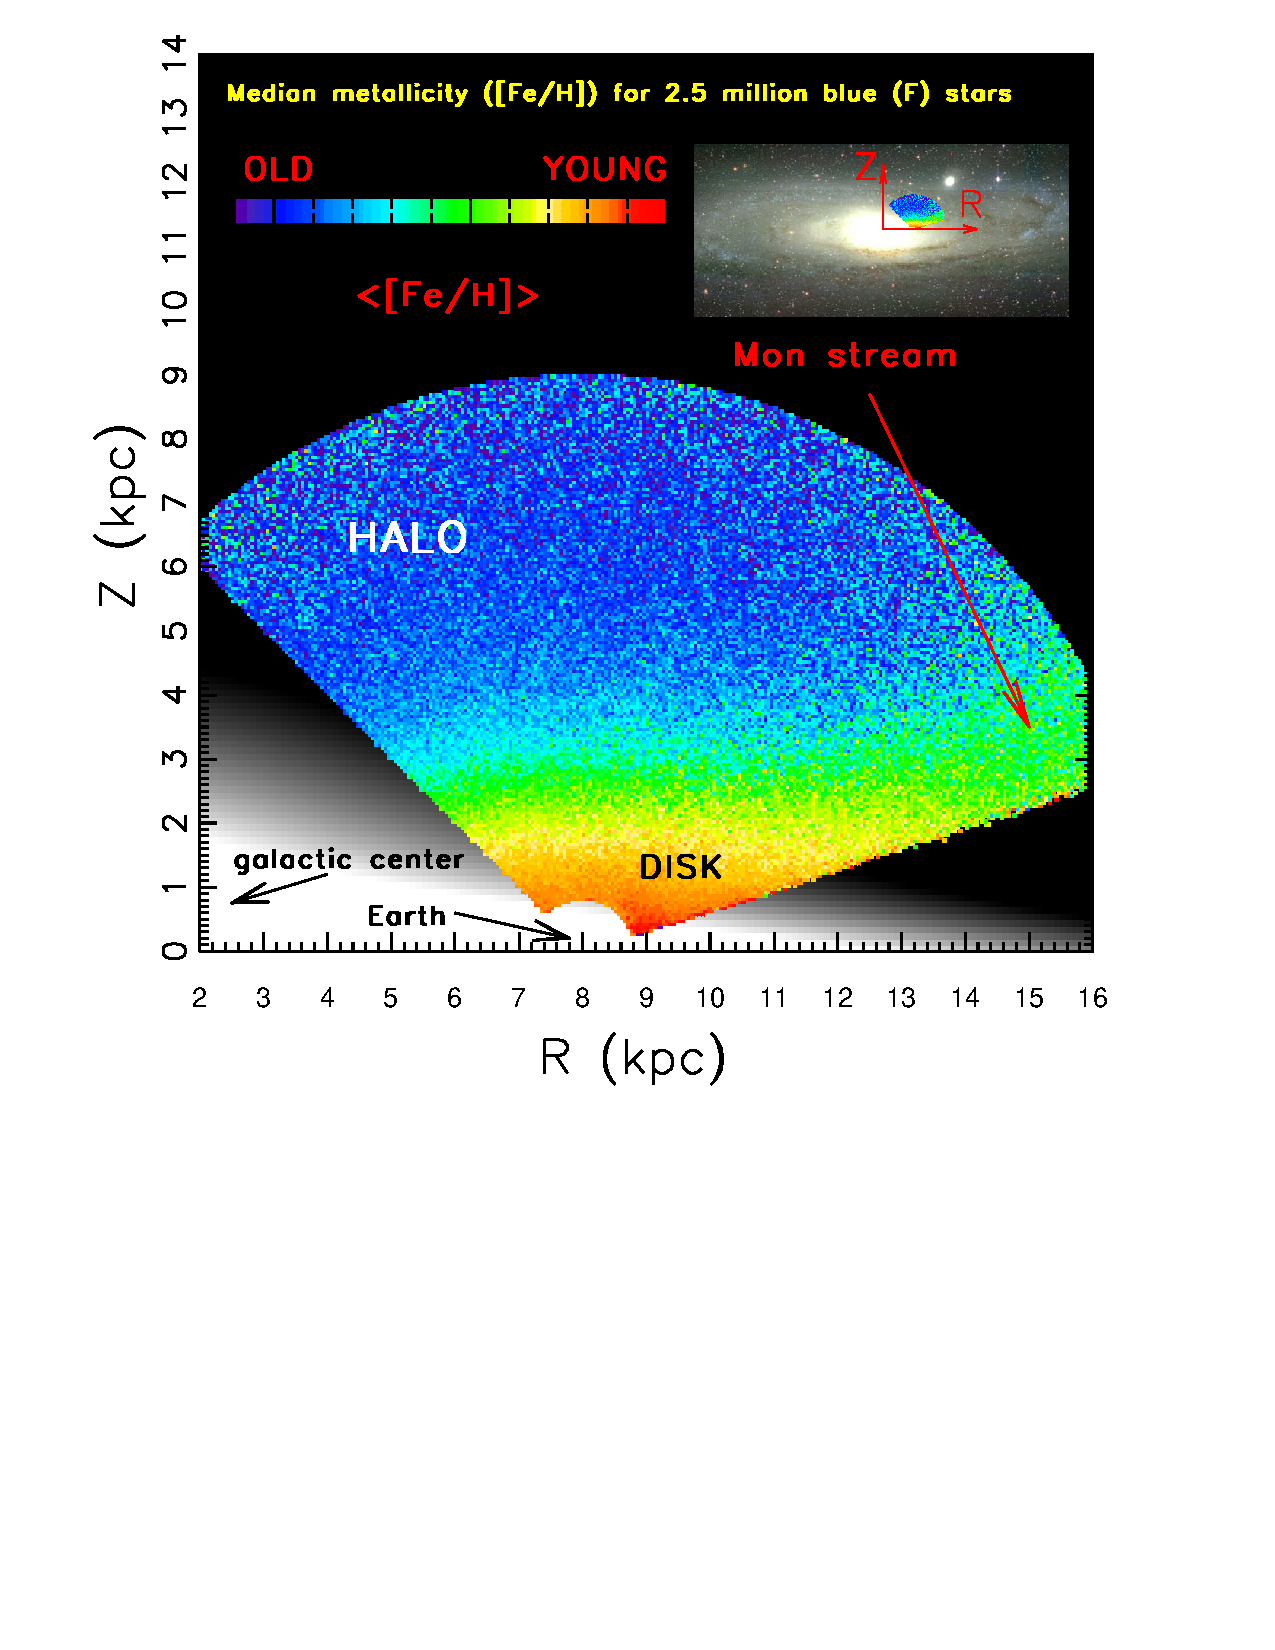
\includegraphics[width=1.0\hsize,clip]{panelsLSST.pdf}
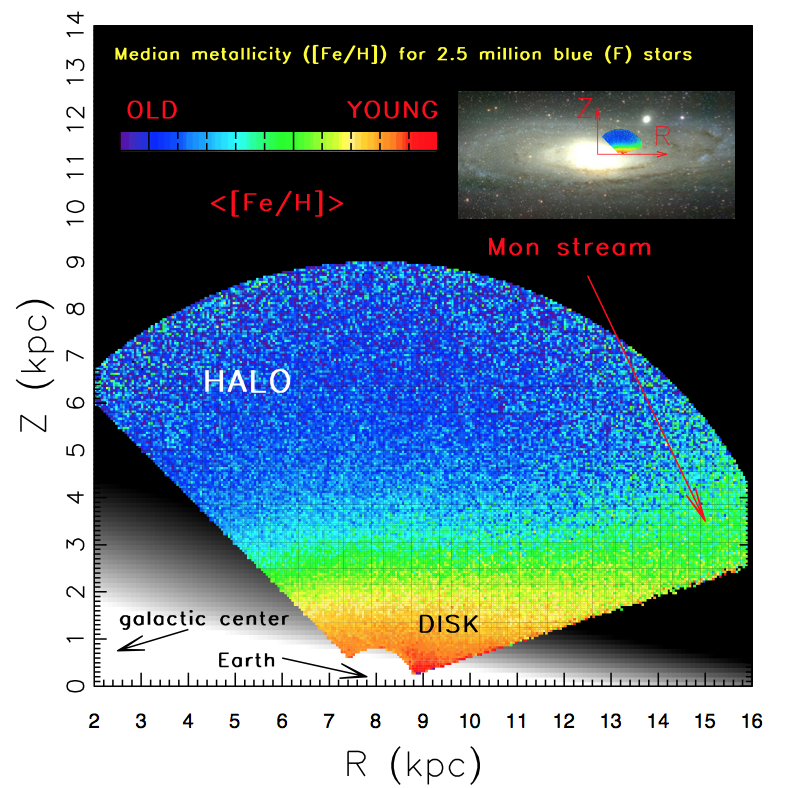
\includegraphics[width=1.\hsize,clip]{panelsLSST.png}
\caption{
The median metallicity map for 2.5 million main-sequence F-type stars within 10 kpc
from the Sun \citep[adapted from][]{2008ApJ...684..287I}. The metallicity is estimated using
$u-g$ and $g-r$ colors measured by SDSS. The position and size of the mapped
region, relative to the rest of the Milky Way, is illustrated in the top right
corner, where the same map is scaled and overlaid on an image of the Andromeda
galaxy. The gradient of the median metallicity is essentially parallel
to the $Z$ axis, except in the Monoceros stream region, as marked. LSST
will extend this map out to 100 kpc, using a sample of over 100 million
main-sequence F stars.}
\label{Fig:FeH3}
\end{figure}


\begin{figure}
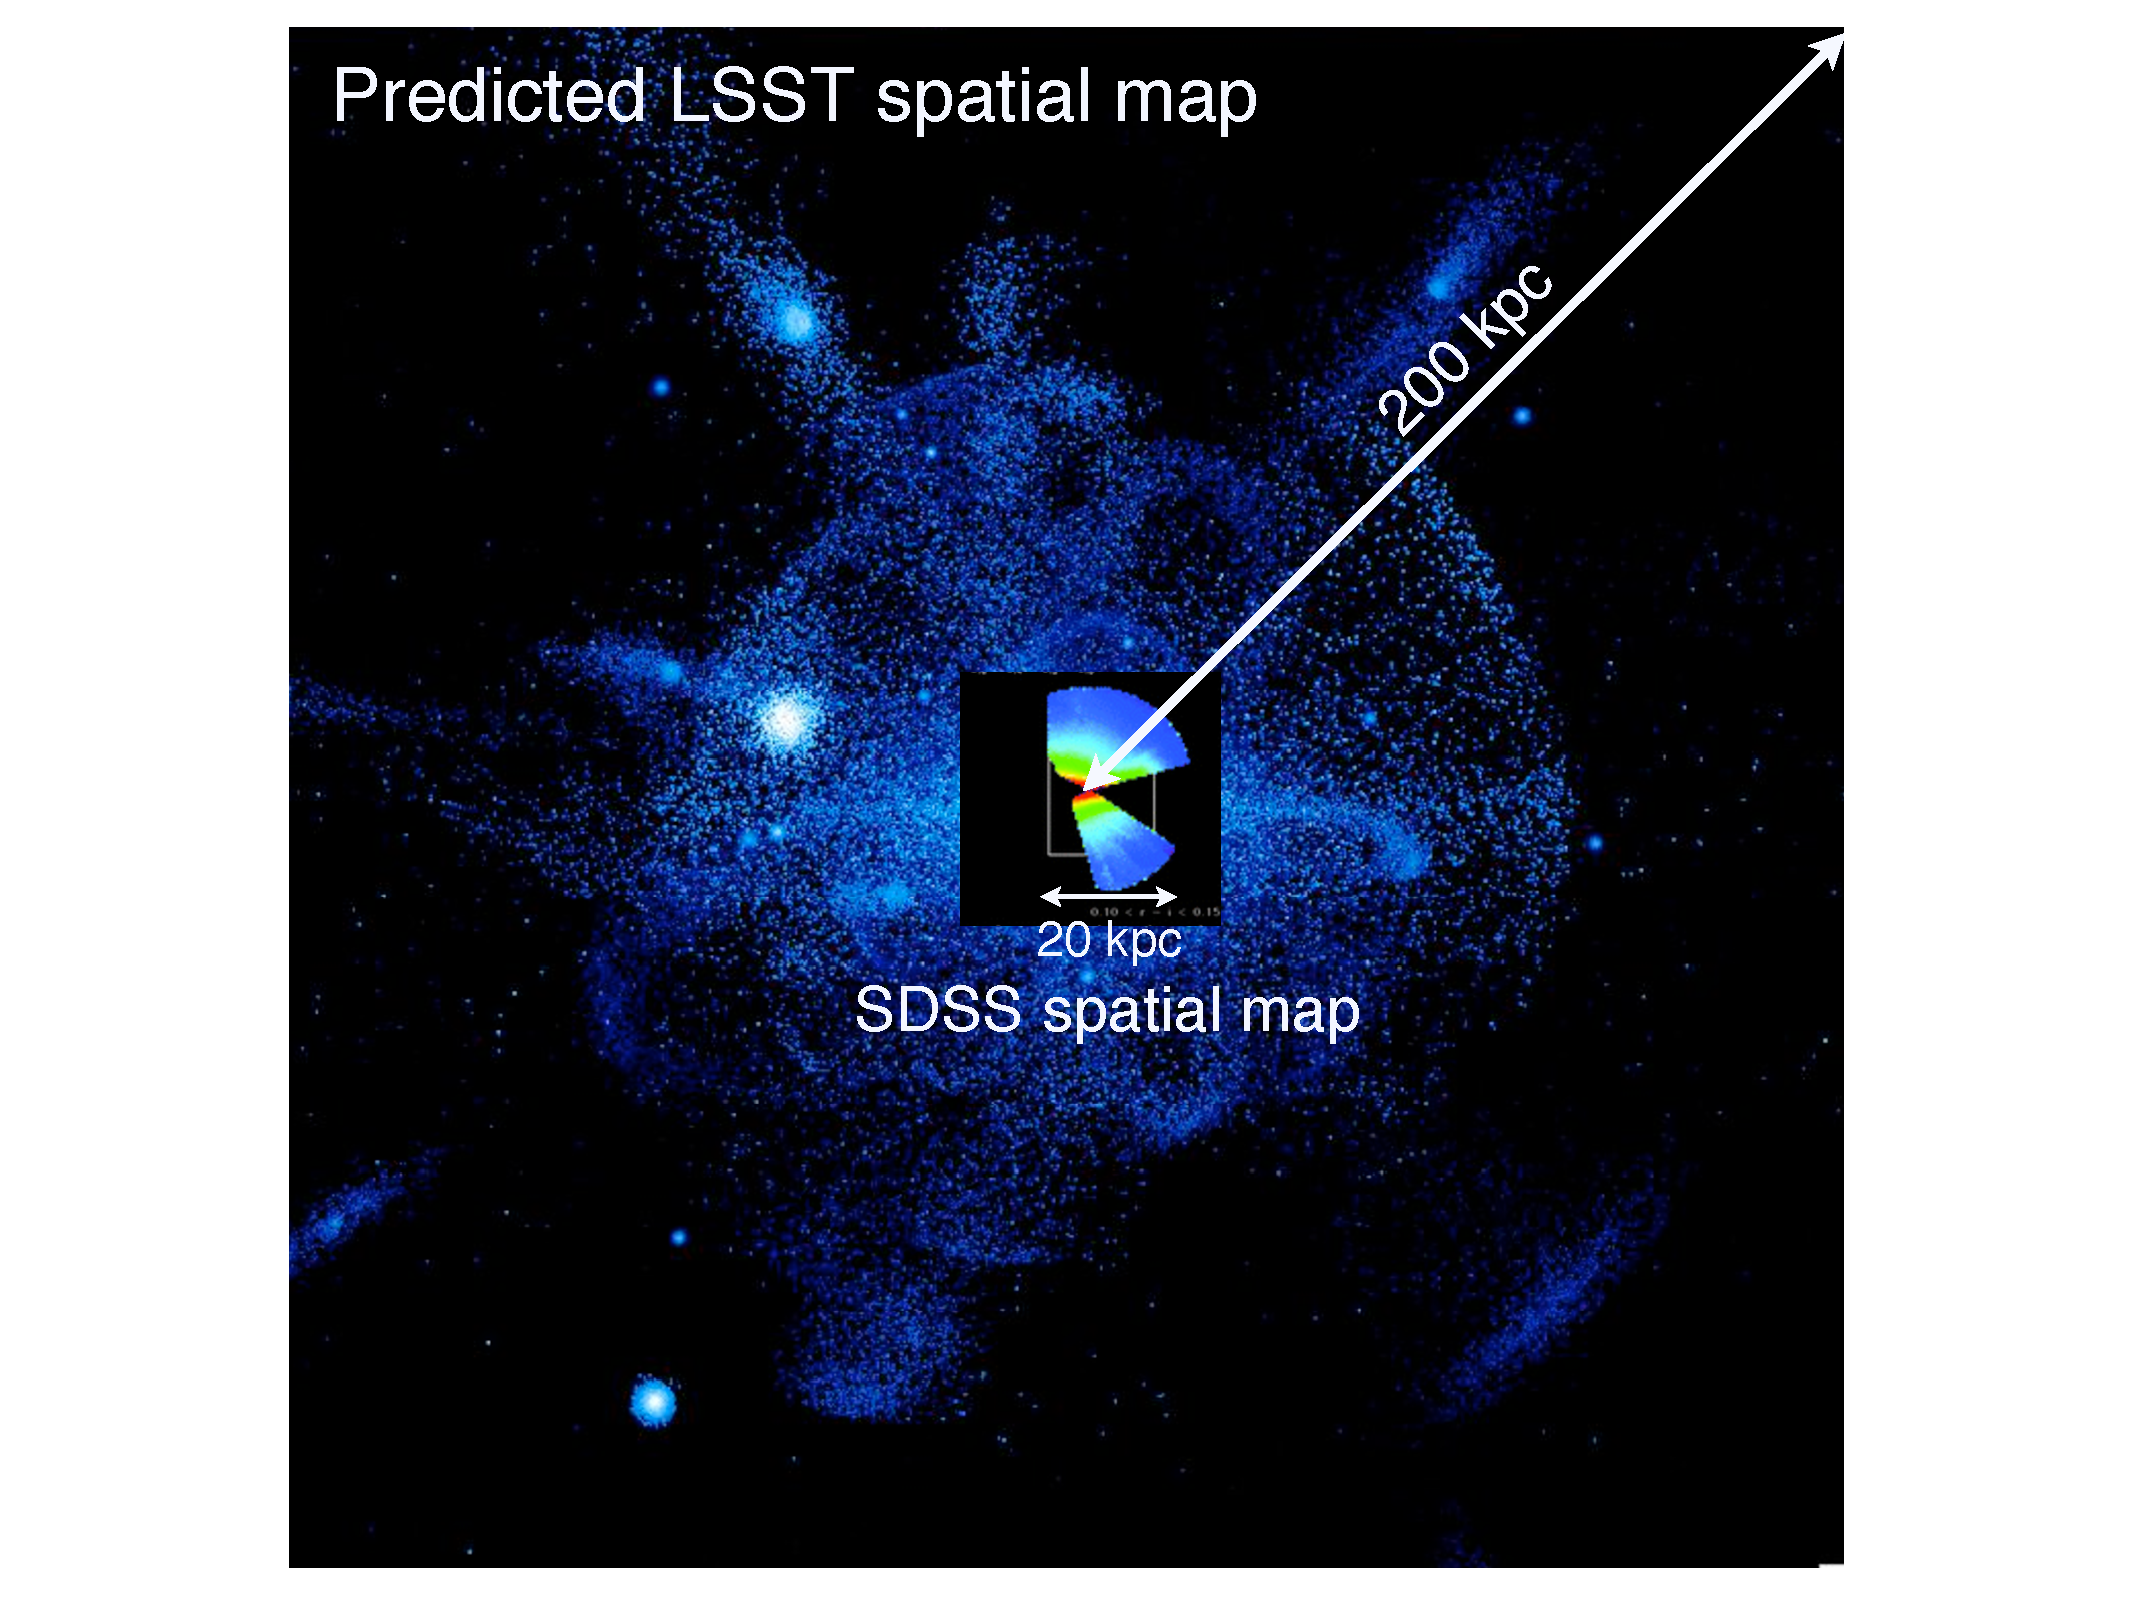
\includegraphics[width=1.\hsize,clip]{BethMWhalo.pdf}
\caption{A predicted spatial distribution of stars out to 150 kpc from the center of the Milky Way,
from \citet{2005ApJ...635..931B}.  LSST will resolve main sequence turnoff stars out to 300 kpc, ten times
more volume than shown here, enabling a high-fidelity spatial map over the entire observed virial volume.
Overlaid on this prediction is the observed SDSS stellar number density map based on main sequence stars
with $0.10 < r-i < 0.15$ \citep{2008ApJ...673..864J}.  This map extends up to $\sim$ 20 kpc from the Sun, with
the white box showing a scale of 20 kpc across and the left side aligned with the Galactic center.
The revolutionary Galaxy map provided by SDSS is only complete to $\sim$40 kpc, or only $\sim$1\% of
the virial volume.  However, the outermost reaches of the stellar halo are predicted to bear the most unique
signatures of our Galaxy's formation \citep{2008ApJ...689..936J,2010MNRAS.406..744C}.   LSST will be the only survey
capable of fully testing such predictions.}
\label{Fig:halo}
\end{figure}



In summary, the LSST data will revolutionize studies of the Milky Way and the entire Local Group. We list a few specific
Galactic science programs that LSST will enable:

\begin{itemize}
\item High-resolution studies of the distribution of stars in the outer halo
          in the six-dimensional space spanned by position, metallicity and proper
          motions \citep[e.g.,][]{2006AJ....132.1768G,2008ApJ...680..295B,2008ApJ...673..864J,2008ApJ...684..287I,2010ApJ...716....1B}.
\item The most complete search possible for halo streams, Galaxy satellites and intra-Local Group
          stars \citep[e.g.][]{2007ApJ...654..897B,2009AJ....137..450W,2014AJ....147...76B}.
\item Deep and highly accurate color-magnitude diagrams for over half of the known
          globular clusters, including tangential velocities from proper motion
          measurements \citep{2008ApJS..179..326A,2007AJ....134..195C}.
\item Mapping the metallicity, kinematics and spatial profile of the Sgr dwarf tidal
          stream \citep[e.g.,][]{2001ApJ...547L.133I,2003ApJ...599.1082M,2005ApJ...619..807L,2014MNRAS.437..116B}
          and the Magellanic stream \citep{2004AJ....128.1606Z}.
\item The measurement of the internal motions of Milky Way dwarf
          galaxies, thereby constraining their density profiles and
	  possibly the nature of dark matter \citep[e.g.,][]{2011ApJ...742...20W}.
\item Detailed constraints on the formation and evolution of the populations within the Galactic Bulge, as traced by the spatial
          distribution, motion, and chemistry of $\sim$10$^{7-8}$ of its stars
          \citep[e.g.][]{2011A&A...534A..80H,2014ApJ...787L..19N}.
\item Studies of the clumpiness of the gravitational potential in the Galaxy using
          fragile wide-angle binaries selected with the aid of trigonometric and
          photometric parallaxes, and common proper motion \cite[e.g.,][]{2004ApJ...601..311Y,2010A&A...509A..46L}.
\item Detailed studies of variable star populations; 2\% or better accurate
          multicolor light curves will be available for a sample of at least 50
          million variable stars \citep{2007AJ....134.2236S}, enabling studies of
          cataclysmic variables, eclipsing binary systems, and rare types of variables.
\item Discovery of rare and faint high proper motion objects: probing the
          faint end of the stellar mass function \citep{2008AJ....135.2177L,2010AJ....140..844F}, and searching for
          free-floating planet candidates \citep{2000MNRAS.314..858L,2014ApJ...786L..18L}.
\item Direct measurement of the faint end of the stellar luminosity function
          using trigonometric parallaxes \citep{2002AJ....124.2721R} and a complete census of the
          solar neighborhood to a distance of 100 pc based on trigonometric parallax measurements for objects as faint as
          $M_r=17$ ($\sim$L5 brown dwarfs). For example, LSST will deliver 10\% or better distances for a sample of about 2,500 stars
          with 18$<M_r<$19. % Comment: (note there are about 400 brown dwarfs with good parallaxes and Gaia will see about 1000,
                                          % but most of these will be early L).
\item The separation of halo M sub-dwarfs from disk M dwarfs, using the $z-y$ color which is sensitive to their rich molecular band
          structure \citep{2011ASPC..448..531W,2013AJ....145...40B}.
\item Studies of white dwarfs using samples of several million objects, including the determination of the halo white dwarf luminosity
          function (SciBook Ch.~6).
\item Measurements of physical properties of stars using large samples of eclipsing binary stars \citep{2013AAS...22111601S}.
\item High-resolution three-dimensional studies of interstellar dust using 5-color
          SEDs of main sequence stars \citep{2011A&A...536A..23P,2012ApJ...757..166B,2014ApJ...783..114G}.
%\item Planetary transits: the data set may include a mini survey of 600
%         deg$^2$ of sky which will collect about 40 hour-long sequences of 200
%          observations each over a 4-month period (see \S~\ref{Sec:minisurveys}).
%          There would be an additional 800 observations over 10 years of these
%          same fields as part of the main survey. With about 10 million or more stars
%          in the sample (depending on where the fields are placed), this would
%          provide excellent base material to study the planet frequency as a
%          function of stellar type, metallicity, and distance from the Galactic plane
%          (e.g., \citep{2000ApJ...529L..45C,Konacki2003}.
\item A census of AGB stars in the Galaxy by searching for resolved envelopes and optical  identifications of IR counterparts
         (e.g., from the WISE survey), and by using long-term variability and color selection \citep{2007ASPC..378..485I}.
\item A complete census of faint populations in nearby star forming regions using
          color and variability selection \citep[e.g.][]{2005AJ....129..907B}.
\end{itemize}


\begin{figure}
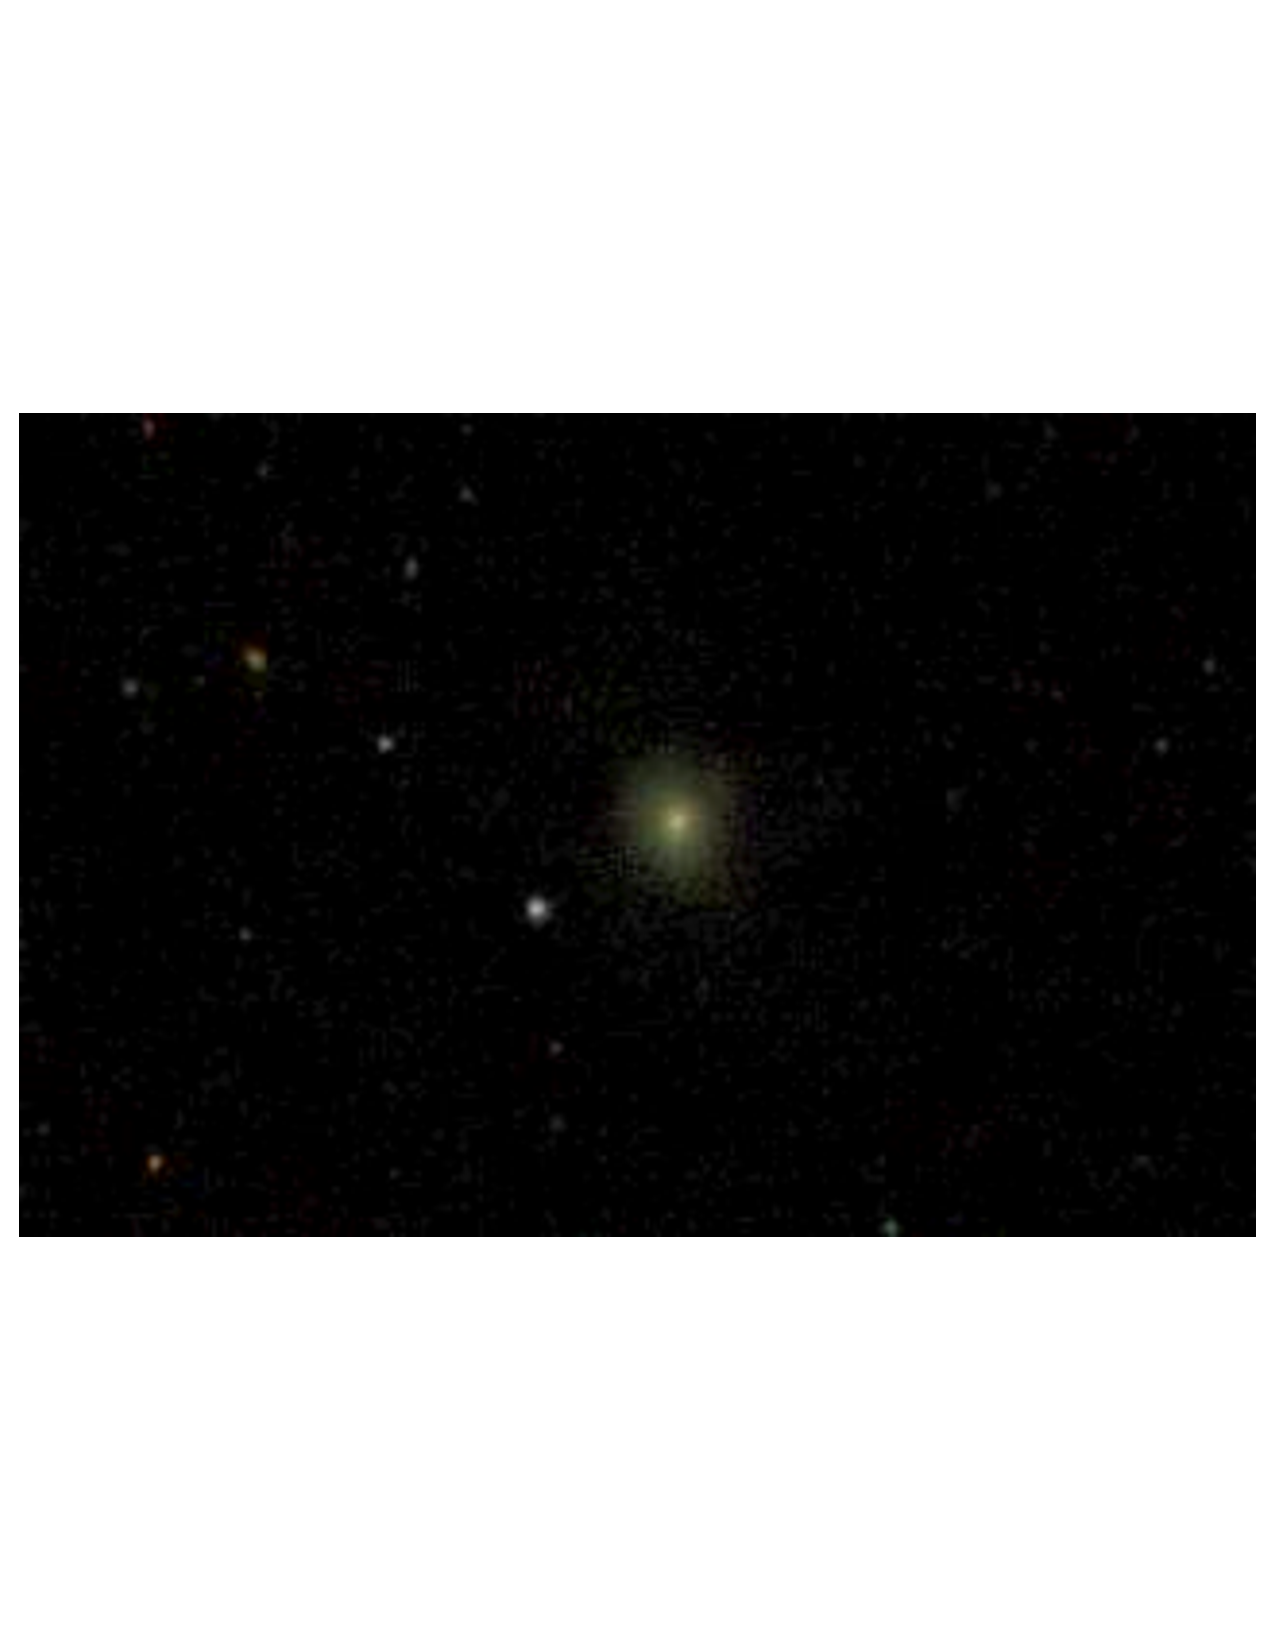
\includegraphics[width=1.0\hsize,clip]{musycSDSS.pdf}
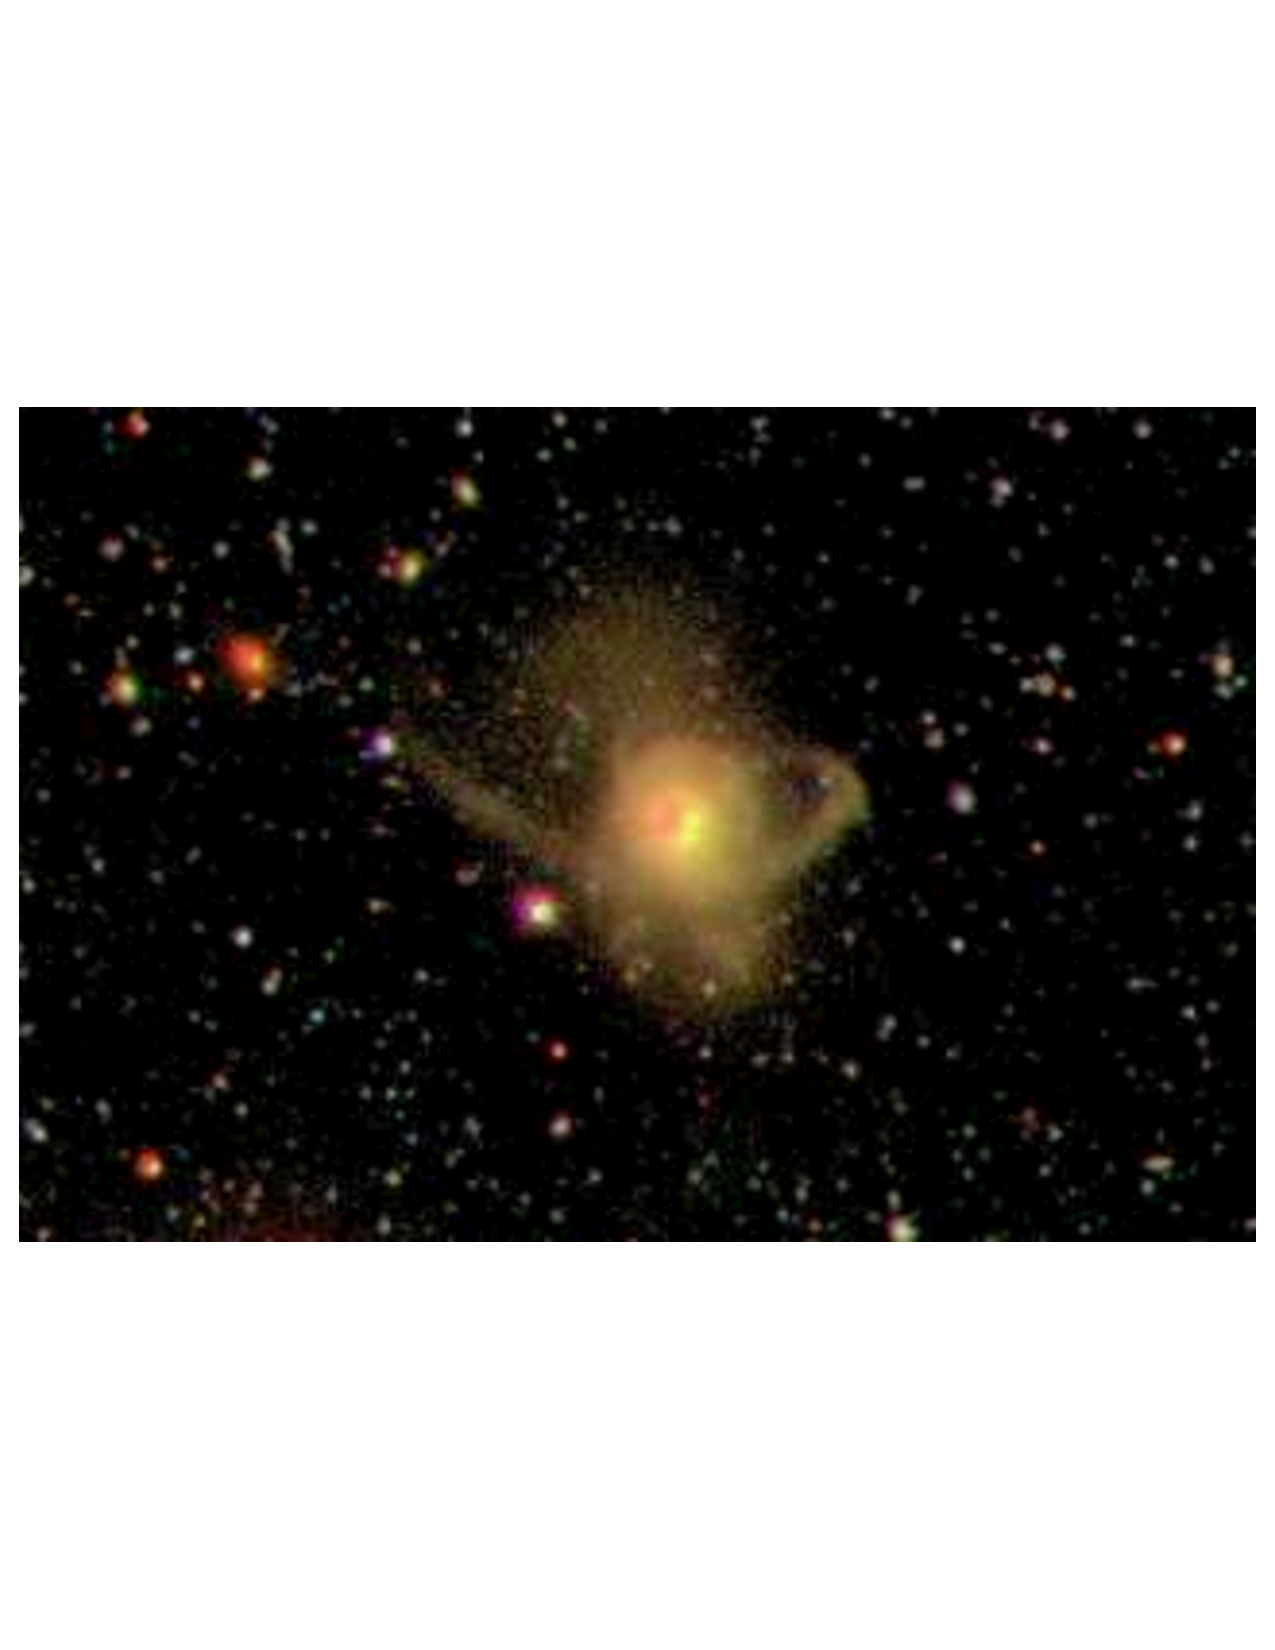
\includegraphics[width=1.0\hsize,clip]{musyc.pdf}
\caption{
A comparison of an SDSS image (2$\times$4 arcmin$^2$ $gri$ composite) showing a typical galaxy at
a redshift of $\sim$0.1 (top) with a similar $BVR$ composite image of the same field obtained by the MUSYC survey
\citep[bottom;][]{2006ApJS..162....1G}. The MUSYC image is about 4 mag deeper than the SDSS image (and about 1 mag less deep
than the anticipated LSST 10-year coadded data). Note the rich surface brightness structure seen in the MUSYC
image that is undetectable in the SDSS image.}
\label{Fig:musyc}
\end{figure}


\subsection{  Additional Science Projects}

The experience with any large survey (e.g., SDSS, 2MASS, VISTA, WISE, GALEX, to name but a
few) is that much of their most interesting science is often unrelated to
the main science drivers, and is often unanticipated at the time the survey is
designed. LSST will enable far more diverse science than encompassed by the
four themes that drive the system design. We list a few anticipated major
programs.

\begin{itemize}
\item Detailed studies of galaxy formation and evolution using their distribution in
luminosity-color-morphology space as a function of redshift. For example, LSST will
enable studies of the rest-frame UV emission, similar to those based on GALEX data
for local galaxies, to a redshift of $\sim$2 for an unprecedentedly large number of
galaxies. These studies project onto many axes:
\begin{itemize}
  \item the evolution of the galaxy luminosity function with redshift, as a function of
        morphology and color;
  \item the evolution of the galaxy color distribution over a wide range of rest-frame
        wavelengths, and as a function of luminosity and morphology;
  \item bulge-disk decomposition, as a function of luminosity and color, over
        a large redshift range;
  \item detailed distribution of satellite galaxies in luminosity-color-morphology space
        as a function of luminosity, color, and morphology of the primary galaxy;
  \item correlations of luminosity, color and morphology with local environment from
           kpc to Mpc scales, and as a function of redshift (see  Figs.~\ref{Fig:musyc} and \ref{Fig:cowan});
  \item the properties of galaxy groups and clusters as a function of cosmic time.
\end{itemize}
\item AGN census to very faint luminosity and a large redshift limit
  \citep{2014IAUS..304...11I}, yielding 20-100 million objects once multiwavelength
      data are used to aid AGN selection (see Fig.~\ref{Fig:panels3}). By reaching substantially further
      down the AGN luminosity function over a very large solid angle, LSST data
      will test evolutionary cosmic downsizing scenarios across the full range of cosmic environments,
      and lead to a much clearer understanding of black-hole growth during the first Gyr. For
      example, LSST should discover $\sim$1000 AGNs at $z\sim6-7.5$,
      representing a dramatic increase over present samples
      \citep[][see also SciBook Ch.~10]{2007AAS...21113709B}.
\item The combination of LSST, Euclid and WFIRST data should allow discovery of at least
       tens of quasars at $z>7.5$ (R. Barnett 2017, priv. comm).
\item LSST data will provide good constraints on AGN lifetimes, or at least the timescales over which
         they make distinct accretion-state transitions, due to large sample
         size and survey lifetime \citep[e.g.][]{2003ApJ...597L.109M}.
\item The first wide field survey of ultra low surface brightness galaxies, with
      photometric redshift information. The currently available samples are highly
      incomplete, especially in the Southern Hemisphere \citep[see Fig.~7 in][]{2007ApJ...654..897B}.
\item Search for strong gravitational lenses to a faint surface
  brightness limit \citep[e.g.][]{1998A&A...330....1B,1998ApJ...498L.107T,2007ApJ...671L...9B}, which can be used to
  explore the dark matter profiles of galaxies \citep[e.g.,][]{2006ApJ...640..662T}.
\end{itemize}


\begin{figure}
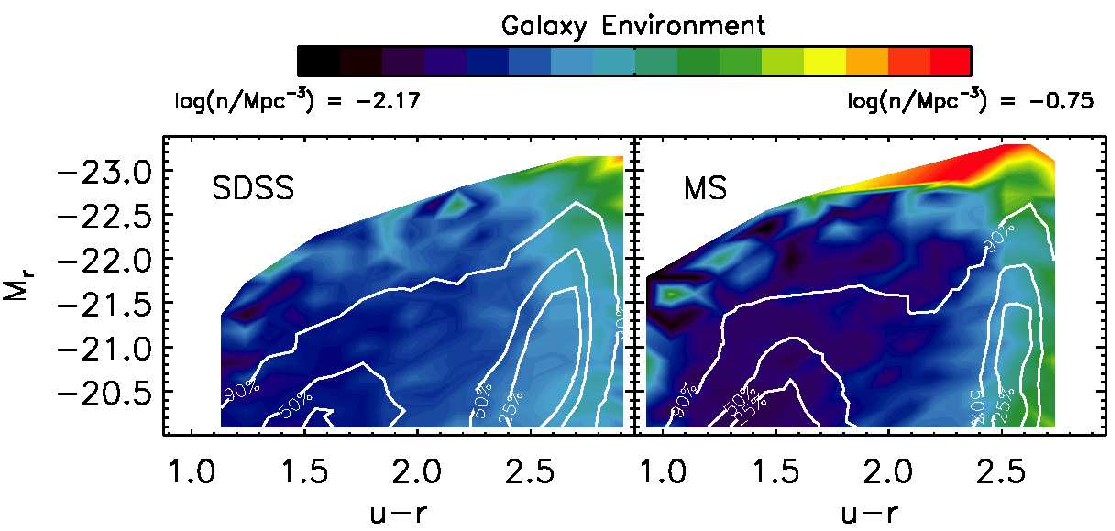
\includegraphics[width=1.0\hsize,clip]{cowan.pdf}
\caption{A comparison of the distribution of galaxies in
luminosity--color--density space measured by SDSS (left) and a model based
on the Millennium simulation (right). The linearly-spaced contours outline
the distribution of a volume-limited sample of galaxies in the plotted diagram, and
the color-coded background shows the median environmental density (computed
using the ten nearest neighbors) for galaxies
with the corresponding luminosity and color. Such multi-variate distributions
encode rich information about formation and evolution of galaxies. Galaxies
detected by SDSS are representative of the low-redshift Universe (the median
redshift is $\sim$0.1). The LSST will enable such studies as a function of
redshift, to $z\sim$2. Adapted from \citet{2008ApJ...674L..13C}.}
\label{Fig:cowan}
\end{figure}


\begin{figure}
%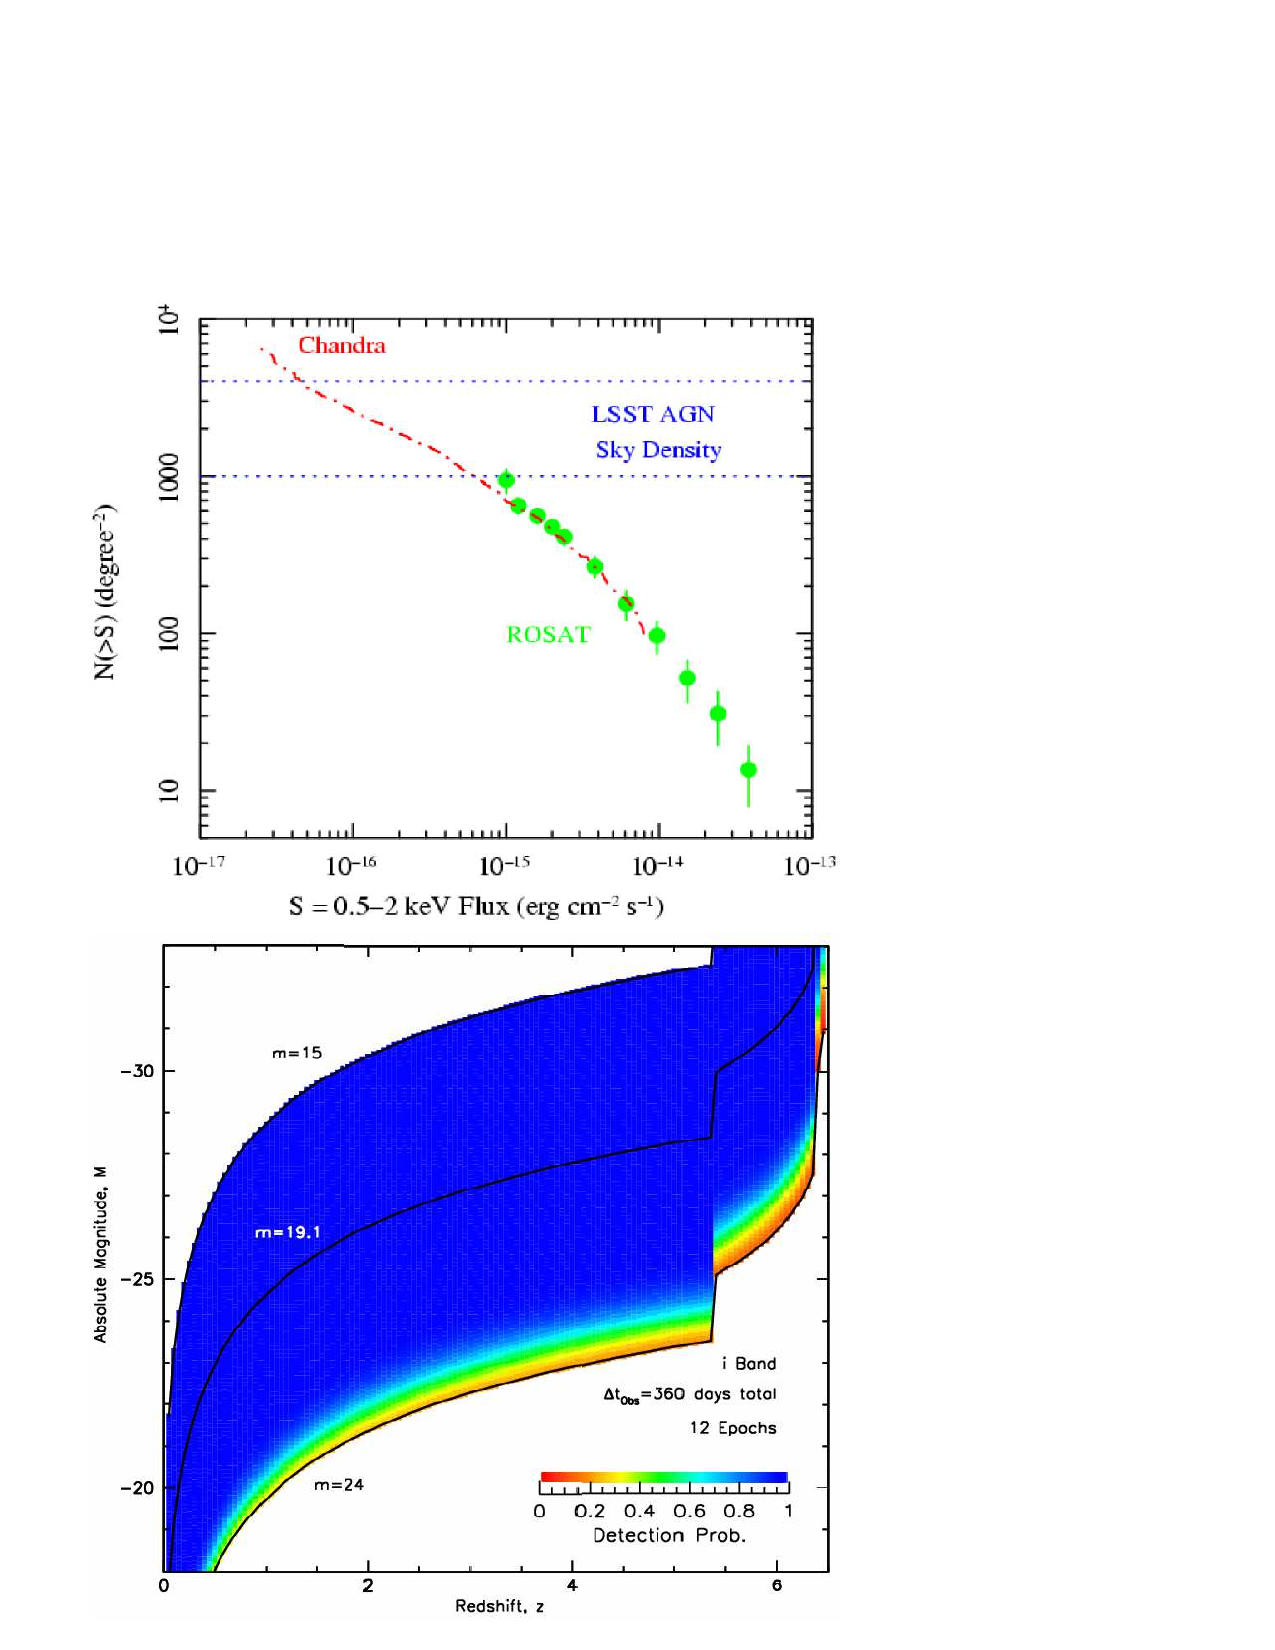
\includegraphics[width=1.0\hsize,clip]{panels3.pdf}
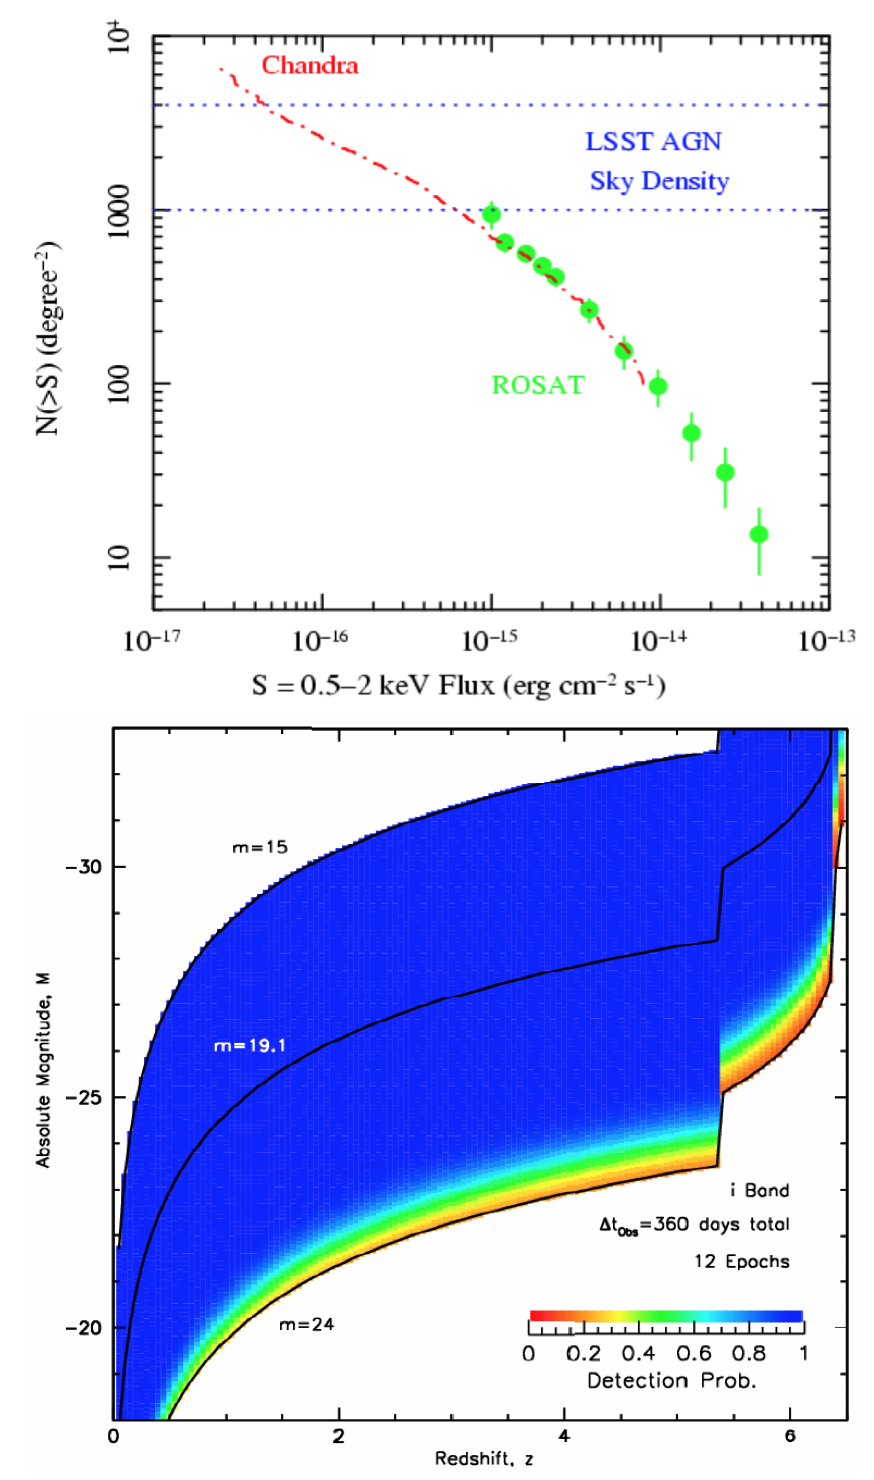
\includegraphics[width=1.0\hsize,clip]{panels3.png}
\caption{The LSST will deliver AGN sky densities of 1000-4000 deg$^{-2}$ (top panel);
The total LSST AGN yield, selected using colors and variability, should be well over
10 million objects, especially once multiwavelength data are also utilized.
The bottom panel shows the expected distribution of these objects in the
absolute magnitude vs. redshift plane, color-coded by the probability for
an object to be
detected as variable after 1 year of observations. Note that quasars will
be detected to their formal luminosity cutoff ($M< -23$) even at redshifts
of $\sim$5. Adapted from \citet{2007AAS...21113709B}.}
\label{Fig:panels3}
\end{figure}

\subsubsection{  Synergy with other projects }

LSST will not operate in isolation and will greatly benefit from other precursor and coeval
data at a variety of wavelengths, depths, and timescales. For example,
in the optical, most of the Celestial
Sphere will be covered to a limit several magnitudes fainter than LSST saturation
($r\sim16$), first by the combination of SDSS, PS1, the Dark Energy Survey \citep{2006SPIE.6269E..2CF} and SkyMapper \citep{2007PASA...24....1K},
and then by the Gaia survey. The SkyMapper survey will obtain imaging data in the southern
sky to similar depths as SDSS, the PS1 surveys provided multi-epoch data deeper
than SDSS in the northern sky, and the Dark Energy Survey will scan
$\sim$5000 deg$^2$ to similar depth as Pan-STARRS in the southern sky. Despite the lack of
the $u$ band data and a depth about a magnitude shallower, the Pan-STARRS surveys
will represent a valuable complement to LSST in providing Northern sky coverage to a limit
fainter than that of SDSS and SkyMapper. LSST and Gaia will
be highly complementary datasets for studying the Milky Way in the multi-dimensional space of
three-dimensional positions, proper motions and metallicity \citep{2012ARA&A..50..251I}.
The Gaia survey will provide calibration checks at the bright end for proper
motions and trigonometric parallax measurements by LSST, and LSST will extend the
Gaia survey by four magnitudes. The upcoming Zwicky Transient Facility \cite[e.g.,][]{2017arXiv170801584L},
with its 600 Megapixel camera and a 47 sq.deg. large field of view, will generate the largest
optical transient stream prior to LSST (at about one tenth of LSST rate) and thus provide
an early insight into astrophysical surprises and technical challenges awaiting LSST.
The LSST data stream will invigorate subsequent investigations by numerous other telescopes
that will provide additional temporal, spectral and spatial resolution coverage.

WFIRST and Euclid will carry out wide-field imaging surveys in the
near-infrared, giving highly complementary photometry to LSST.  The
resulting galaxy SEDs should give rise to even better photometric
redshifts, as well as tighter constraints on stellar masses and star
formation histories crucial for galaxy evolution studies.  The weak
lensing analyses from space and from the ground will also be highly
complementary, and will provide crucial cross-checks of one another.
LSST also presents the opportunity to conduct simultaneous observations
of WFIRST's Galactic Bulge survey fields, from which it will be possible to
measure the parallax and hence the lens masses for most microlensing
events, as well as providing valuable lightcurve coverage during the large
data gaps between WFIRST survey `seasons'.

LSST will also enable multi-wavelength studies of faint optical
sources using gamma-ray, X-ray, IR and radio data.  For example, the
SDSS detected only 1/3 of all 20cm FIRST sources \citep{1995ApJ...450..559B}
because it was too shallow by $\sim$4 mag for a complete optical
identification. Similarly, deep optical data are required for
identification of X-ray sources \citep{2005ARA&A..43..827B,2017AN....338..241B}.

LSST will provide a crucial complementary capability to space
experiments operating in other wavebands, such as the
%Black Hole Finder Einstein Probe
NuSTAR Mission \citep{2013ApJ...770..103H},
%\footnote{http://www.nustar.caltech.edu/},
eROSITA \citep{2012arXiv1209.3114M},
and the \textit{Fermi}
Gamma-ray Space Telescope \cite[e.g.,][]{2009ApJ...697.1071A}.
%The Laser Interferometer Space Antenna (LISA) and the
The Laser Interferometer Gravitational
Wave Observatory (LIGO) has now detected ultracompact binaries and black-hole mergers through the
gravitational wave outbursts that are emitted during the final stages of such events.
LSST will also aid studies of  the electromagnetic signal that accompanies the gravitational wave emission,
thereby providing an accurate position on the sky for the system, which is
crucial for subsequent observations. LSST will also add new value to the archives for
billion-dollar class space missions such as Chandra, XMM-Newton, Spitzer, Herschel,
etc., because deep optical multi-color data will enable
massive photometric  studies of sources from these missions;
any areas of the sky -- whether by design or by serendipity -- in which past, present, or future
multiwavelength surveys overlap with LSST sky coverage, will be further promoted by LSST
investigations to ``optical plus multiwavelength Selected Areas''.
Last but not least, the huge samples of various astronomical source
populations will yield extremely rare objects for investigations by powerful
facilities such as JWST \citep{2006SSRv..123..485G} and the next generation
of 20-40 meter telescopes.
%GSMT \citep{Kan2003}.

In summary, the diversity of science enabled by LSST will be
unparalleled, extending from the physics of gravity and the
early Universe to the properties of ``killer'' asteroids. While
there are other projects that aim to address some of the same
science goals, no other project matches this diversity and
LSST's potential impact on society in general.
